%%%%%%%%%%%%%%
%% Run LaTeX on this file several times to get Table of Contents,
%% cross-references, and citations.

%% If you have font problems, you may edit the w-bookps.sty file
%% to customize the font names to match those on your system.

%% w-bksamp.tex. Current Version: Feb 16, 2012
%%%%%%%%%%%%%%%%%%%%%%%%%%%%%%%%%%%%%%%%%%%%%%%%%%%%%%%%%%%%%%%%
%
%  Sample file for
%  Wiley Book Style, Design No.: SD 001B, 7x10
%  Wiley Book Style, Design No.: SD 004B, 6x9
%
%
%  Prepared by Amy Hendrickson, TeXnology Inc.
%  http://www.texnology.com
%%%%%%%%%%%%%%%%%%%%%%%%%%%%%%%%%%%%%%%%%%%%%%%%%%%%%%%%%%%%%%%%

%%%%%%%%%%%%%
% 7x10
%\documentclass{wileySev}

% 6x9
\documentclass{wileySix}

\usepackage{graphicx}
\usepackage{listings}
\usepackage{float}
\usepackage[urlcolor=blue, colorlinks=true]{hyperref}
\usepackage{textcomp}
\usepackage{gensymb}
\usepackage{color}
 
\definecolor{codegreen}{rgb}{0,0.6,0}
\definecolor{codegray}{rgb}{0.5,0.5,0.5}
\definecolor{codepurple}{rgb}{0.58,0,0.82}
\definecolor{backcolour}{rgb}{0.95,0.95,0.92}
 
\lstdefinestyle{mystyle}{
    backgroundcolor=\color{backcolour},   
    commentstyle=\color{codegreen},
    keywordstyle=\color{magenta},
    numberstyle=\tiny\color{codegray},
    stringstyle=\color{codepurple},
    basicstyle=\footnotesize,
    breakatwhitespace=false,         
    breaklines=true,                 
    captionpos=b,                    
    keepspaces=true,                 
    numbers=left,                    
    numbersep=5pt,                  
    showspaces=false,                
    showstringspaces=false,
    showtabs=false,                  
    tabsize=2,
    language=sh
}
 
\lstset{style=mystyle}

%%%%%%%
%% for times math: However, this package disables bold math (!)
%% \mathbf{x} will still work, but you will not have bold math
%% in section heads or chapter titles. If you don't use math
%% in those environments, mathptmx might be a good choice.

% \usepackage{mathptmx}

% For PostScript text
\usepackage{w-bookps}

%%%%%%%%%%%%%%%%%%%%%%%%%%%%%%%%%%%%%%%%%%%%%%%%%%%%%%%%%%%%%%%%
%% Other packages you might want to use:

% for chapter bibliography made with BibTeX
% \usepackage{chapterbib}

% for multiple indices
% \usepackage{multind}

% for answers to problems
% \usepackage{answers}

%%%%%%%%%%%%%%%%%%%%%%%%%%%%%%
%% Change options here if you want:
%%
%% How many levels of section head would you like numbered?
%% 0= no section numbers, 1= section, 2= subsection, 3= subsubsection
%%==>>
\setcounter{secnumdepth}{3}

%% How many levels of section head would you like to appear in the
%% Table of Contents?
%% 0= chapter titles, 1= section titles, 2= subsection titles, 
%% 3= subsubsection titles.
%%==>>
\setcounter{tocdepth}{2}

%% Cropmarks? good for final page makeup
%% \docropmarks

%%%%%%%%%%%%%%%%%%%%%%%%%%%%%%
%
% DRAFT
%
% Uncomment to get double spacing between lines, current date and time
% printed at bottom of page.
% \draft
% (If you want to keep tables from becoming double spaced also uncomment
% this):
% \renewcommand{\arraystretch}{0.6}
%%%%%%%%%%%%%%%%%%%%%%%%%%%%%%

%%%%%%% Demo of section head containing sample macro:
%% To get a macro to expand correctly in a section head, with upper and
%% lower case math, put the definition and set the box 
%% before \begin{document}, so that when it appears in the 
%% table of contents it will also work:

\newcommand{\VT}[1]{\ensuremath{{V_{T#1}}}}

%% use a box to expand the macro before we put it into the section head:

\newbox\sectsavebox
\setbox\sectsavebox=\hbox{\boldmath\VT{xyz}}

%%%%%%%%%%%%%%%%% End Demo


\begin{document}


\booktitle{Cerdas Menguasai Git}
\subtitle{Dalam 24 Jam}

\authors{Rolly M. Awangga\\
\affil{Informatics Research Center}
%Floyd J. Fowler, Jr.\\
%\affil{University of New Mexico}
}

\offprintinfo{Cerdas Menguasai Git, First Edition}{Rolly M. Awangga}

%% Can use \\ if title, and edition are too wide, ie,
%% \offprintinfo{Survey Methodology,\\ Second Edition}{Robert M. Groves}

%%%%%%%%%%%%%%%%%%%%%%%%%%%%%%
%% 
\halftitlepage

\titlepage


\begin{copyrightpage}{2019}
%Survey Methodology / Robert M. Groves . . . [et al.].
%\       p. cm.---(Wiley series in survey methodology)
%\    ``Wiley-Interscience."
%\    Includes bibliographical references and index.
%\    ISBN 0-471-48348-6 (pbk.)
%\    1. Surveys---Methodology.  2. Social 
%\  sciences---Research---Statistical methods.  I. Groves, Robert M.  II. %
%Series.\\
%
%HA31.2.S873 2007
%001.4'33---dc22                                             2004044064
\end{copyrightpage}

\dedication{`Jika Kamu tidak dapat menahan lelahnya belajar, 
Maka kamu harus sanggup menahan perihnya Kebodohan.'
~Imam Syafi'i~}

\begin{contributors}
\name{Rolly Maulana Awangga,} Informatics Research Center., Politeknik Pos Indonesia, Bandung,
Indonesia



\end{contributors}

\contentsinbrief
\tableofcontents
\listoffigures
\listoftables
\lstlistoflistings


\begin{foreword}
Sepatah kata dari Kaprodi, Kabag Kemahasiswaan dan Mahasiswa
\end{foreword}

\begin{preface}
Buku ini diciptakan bagi yang awam dengan git sekalipun.

\prefaceauthor{R. M. Awangga}
\where{Bandung, Jawa Barat\\
Februari, 2019}
\end{preface}


\begin{acknowledgments}
Terima kasih atas semua masukan dari para mahasiswa agar bisa membuat buku ini 
lebih baik dan lebih mudah dimengerti.

Terima kasih ini juga ditujukan khusus untuk team IRC yang 
telah fokus untuk belajar dan memahami bagaimana buku ini mendampingi proses 
Intership.
\authorinitials{R. M. A.}
\end{acknowledgments}

\begin{acronyms}
\acro{ACGIH}{American Conference of Governmental Industrial Hygienists}
\acro{AEC}{Atomic Energy Commission}
\acro{OSHA}{Occupational Health and Safety Commission}
\acro{SAMA}{Scientific Apparatus Makers Association}
\end{acronyms}

\begin{glossary}
\term{git}Merupakan manajemen sumber kode yang dibuat oleh linus torvald.

\term{bash}Merupakan bahasa sistem operasi berbasiskan *NIX.

\term{linux}Sistem operasi berbasis sumber kode terbuka yang dibuat oleh Linus Torvald
\end{glossary}

\begin{symbols}
\term{A}Amplitude

\term{\hbox{\&}}Propositional logic symbol 

\term{a}Filter Coefficient

\bigskip

\term{\mathcal{B}}Number of Beats
\end{symbols}

\begin{introduction}

%% optional, but if you want to list author:

\introauthor{Rolly Maulana Awangga, S.T., M.T.}
{Informatics Research Center\\
Bandung, Jawa Barat, Indonesia}

Pada era disruptif  \index{disruptif}\index{disruptif!modern} 
saat ini. git merupakan sebuah kebutuhan dalam sebuah organisasi pengembangan perangkat lunak.
Buku ini diharapkan bisa menjadi penghantar para programmer, analis, IT Operation dan Project Manajer.
Dalam melakukan implementasi git pada diri dan organisasinya.

Rumusnya cuman sebagai contoh aja biar keren\cite{awangga2018sampeu}.

\begin{equation}
ABC {\cal DEF} \alpha\beta\Gamma\Delta\sum^{abc}_{def}
\end{equation}

\end{introduction}

%%%%%%%%%%%%%%%%%%Isi Buku_

\chapter{Chapter 1}
\section{1174006 - Kadek Diva Krishna Murti}

\subsection{Teori}
\subsubsection{Definisi Kecerdasan Buatan}
\hfill\break
Kecerdasan buatan atau artificial intelligence (AI) menurut beberapa pakar adalah sebagai berikut:
\begin{enumerate}
	\item Schalkoff (1990): AI adalah bidang studi yang mencoba meniru dan menerangkan perilaku cerdas yang dilakukan oleh manusia dalam bentuk proses komputasi.
	\item Rich dan Knight (1991): AI adalah studi tentang cara membuat komputer melakukan sesuatu yang sampai saat ini orang dapat melakukannya lebih baik.
	\item Luger dan Stubblefield (1993): AI adalah cabang ilmu komputer yang berhubungan dengan otomasi perilaku yang cerdas.
	\item Keen dan Haag (1996): AI adalah cabang ilmu komputer yang berkaitan dengan pemodelan, penangkapan, dan penyimpanan kecerdasan manusia ke dalam sebuah sistem teknologi informasi sehingga sistem tersebut nantinya dapat memfasilitasi dalam melakukan pengambilan keputusan yang biasanya dilakukan oleh manusia.
\end{enumerate}
\noindent
Jadi dapat disimpulkan kecerdasan buatan atau artificial intelligence (AI) merupakan salah satu bagian ilmu komputer yang membuat mesin (komputer) dapat melakukan pekerjaan seperti dan sebaik yang dilakukan oleh manusia. Seperti yang kita tahu pada awal diciptakannya, komputer hanya difungsikan sebagai alat hitung saja. Namun seiring dengan perkembangan jaman, maka peran komputer semakin mendominasi kehidupan umat manusia. Komputer tidak lagi sekedar digunakan sebagai alat hitungn namun diharapkan untuk dapat diberdayakan untuk mengerjakan segala sesuatu yang bisa dikerjakan oleh manusia.

\subsubsection{Sejarah dan Perkembangan Kercerdasan Buatan}
\hfill\break
Istilah AI pertama kali dikemukakan pada tahun 1956 dikonferensi Darthmouth. Sejak saat itu AI terus dikembangkan sebab berbagai penelitian mengenai teori-teori dan prinsip-prinsipnya juga terus berkembang. Meskipun istilah AI baru muncul tahun 1956, tetapi teori-teori mengarah ke AI sudah muncul sejak tahun 1941. Berikut ini tahapan-tahapan sejarah perkembangan AI:
\begin{enumerate}
	\item Era Komputer Elektronik (1941)
	\hfill\break
	Pada tahun 1941 telah ditemukan alat penyimpanan dan pemrosesan informasi. Penemuan tersebut dinamakan komputer elektronik yang dikembangkan di USA dan Jerman. Komputer pertama ini memerlukan ruangan yang luas dan ruang AC yang terpisah. Saat itu komputer meibatkan konfigurasi ribuan kabel untuk menjalankan suatu program. Hal ini sangat merepotkan bagi para programmer. Pada tahun 1949, berhasil dibuat komputer yang mampu menyimpan program sehingga membuat pekerjaan untuk memasukkan program menjadi lebih mudah. Penemuan ini menjadi dasar pengembangan program yang mengarah ke AI.

	\item Masa Persiapan AI (1943–1956)
	\hfill\break
	Pada tahun 1943, Warren McCulloch dan Walter Pitts mengemukakan tiga hal: pengetahuan fisiologi dasar dan fungsi sel syaraf dalam otak, analisis formal tentang logika proporsi (propositional logic), dan teori komputasi turing. Mereka berhasil membuat suatu model syaraf tiruan (artificial neuron) di mana setiap neuron digambarkan sebagai on dan off. Mereka menunjukkan bahwa setiap fungsi dapat dihitung dengan suatu jaringan sel syaraf dan bahwa semua hubungan logis dapat diimplementasikan dengan struktur jaringan yang sederhana.
	\noindent
	Pada tahun 1950, Norbert Wiener mebuat penelitian mengenai prinsip-prinsip teori feedback. Contoh yang terkenal adalah thermostat. Penemuan ini juga merupakan awal perkembangan AI. Pada tahun 1956, John McCarthy (yang setelah lulus dari Princeton kemudian melanjutkan ke Dartmouth College) meyakinkan Minsky, Claude Shannon dan Nathaniel Rochester untuk membantunya melakukan penelitian dalam bidang Automata, jaringan sel syaraf dan pembelajaran intelejensia. Mereka mengerjakan proyek ini selama dua bulan di Dartmouth. Hasilnya adalah program yang mampu ber-pikir non-numerik dan menyelesaikan masalah pemikiran, yang dinamakan Principia Mathematica. Hal ini menjadikan McCarthy disebut sebagai Father of AI (Bapak AI).

	\item Awal Perkembangan AI (1952–1969)
	\hfill\break
	Pada tahun-tahun pertama pengembangannya, AI mengalami banyak kesuksesan. Diawali dengan kesuksesan Newell dan Simon dengan sebuah program yang disebut General Problem Solver. Program ini dirancang untuk memulai penyelesaian masalah secara manusiawi. Pada tahun 1958, McCarthy di MTT Lab Memo No. 1 mendefinisikan bahasa pemrograman tingkat tinggi yaitu LISP, yang sekarang mendominasi pembuatan program-program AI. Kemudian, McCarthy membuat program yang dinamakan Programs With Common Sense. Di dalam program tersebut, dibuat rancangan untuk menggunakan pengetahuan dalam mencari solusi. Pada tahun 1959, Nathaniel Rochester dari IBM dan mahasiswa-mahasiswanya mengeluarkan program AI Geometry Theorm Prover. Program ini dapat membuktikan suatu teorema menggunakan axioma-axioma yang ada. Pada tahun 1963, program yang dibuat James Slagle mampu menyelesaikan masalah integral tertutup untuk mata kuliah kalkulus. Pada tahun 1968, program analogi buatan Tom Evan menyelesaikan masalah analogi geometris yang ada pada tes IQ.

	\item Perkembangan AI Melambat (1966–1974)
	\hfill\break
	Prediksi Herbert Simon pada tahun 1957 yang menyatakan bahwa AI akan menjadi ilmu pengetahuan yang akan berkembang dengan pesat ternyata meleset. Pada 10 tahun kemudian, perkembangan AI melambat. Hal ini disebabkan adanya 3 kesulitan utama yang dihadapi AI, yaitu:
	\begin{enumerate}
		\item Masalah pertama: program-program AI yang bermunculan hanya mangandung sedikit atau bahkan tidak mengandung sama sekali pengetahuan (knowledge) pada subjeknya. Program-program AI berhasil hanya karena manipulasi sintetis yang sederhana. Sebagai contoh adalah Weizenbaum’s ELIZA program (1965) yang dapat melakukan percakapan serius pada berbagai topik, sebenarnya hanyalah peminjaman dan manipulasi kalimat-kalimat yang diketikkan oleh manusia.
		\item Masalah kedua: banyak masalah yang harus diselesaikan oleh AI. Karena terlalu banyaknya masalah yang berkaitan, maka tidak jarang banyak terjadi kegagalan pada pembuatan program AI.
		\item Masalah ketiga: ada beberapa batasan pada struktur dasar yang digunakan untuk menghasilkan perilaku intelejensia. Sebagai contoh adalah pada tahun 1969 buku Minsky dan Papert Perceptrons membuktikan bahwa program-program perceptrons dapat mempelajari segala sesuatu, tetapi program-program tersebut hanya mempresentasikan sejumlah kecil saja. Sebagai contoh dua masukan perceptrons yang berbeda tidak dapat dilatihkan untuk mengenali kedua masukan yang berbeda tersebut.
	\end{enumerate}

	\item Sistem Berbasis Pengetahuan (1969–1979)
	\hfill\break
	Pengetahuan adalah kekuatan pendukung AI. Hal ini dibuktiikan dengan program yang dibuat oleh Ed Feigenbaum,Bruce Buchanan dan Joshua Lederberg yang membuat program untuk memecahkan masalah struktur molekul dari informasi yang didapatkan dari spectometer massa. Program ini dinamakan Dendral programs yang berfokus pada segi pengetahuan kimia. Dari segi diagnosis media juga sudah ada yang menemukannya, yaitu Saul Amarel dalam proyek computer in biomedicine. Proyek ini diawali dari keinginan untuk mendapatkan diagnosa penyakit berdasarkan pengetahuan yang ada pada mekanisme penyebab proses penyakit.

	\item AI Menjadi Sebuah Industri (1980–1988)
	\hfill\break
	Industrialisasi AI diawali dengan ditemukannya expert system (sistem pakar) yang dinamakan R1 yang mampu mengkonfigurasi sistem-sistem komputer baru. Program tersebut mulai dioperasikan di Digital Equipment Corporation(DEC), McDermott, pada tahun 1982. Pada tahun 1986, program ini telah berhasil menghemat US\$40 juta per tahun. Pada tahun 1988, kelompok AI di DEC menjalankan 40 sistem pakar. Hampir semua perusahaan besar di USA mempunyai divisi AI sendiri yang menggunakan ataupun mempelajari sistem pakar. Booming industri AI ini juga melibatkan perusahaan-perusahaan besar seperti Carnegie Group, Inference, Intellicorp, dan Technoledge yang menawarkan software tools untuk membangun sistem pakar. Perusahaan hardware seperti LISP dan Machines Inc., Texas Instruments, Symbolics, dan Xerox juga turut berperan dalam membangun workstation yang dioptimasi untuk pembangunan program LISP. Sehingga, perusahaan yang sejak tahun 1982 hanya menghasilkan beberapa juta US dolar per tahun meningkat menjadi 2 milyar US dolar per tahun pada tahun 1988.

	\item Kembalinya Jaringan Syaraf Tiruan (1986–Sekarang)
	\hfill\break
	Meskipun bidang ilmu komputer menolak jaringan syaraf tiruan setelah diterbitkannya buku "perceptrons" karangan Minsky dan Papert, tetapi para ilmuan masih mempelajari bidang ilmu tersebut dari sudut pandang yang lain yaitu fisika. Para ahli seperti Hopfield (1982) menggunakan teknik-teknik mekanika statistika untuk menganalisa sifat-sifat penyimpanan dan optimasi pada jaringan syaraf. Para ahli psikollogi, David Rumelhart dan Geoff Hinton, melanjutkan penelitian mengenai model syaraf pada memori. Pada tahun 1985-an sedikitnya empat kelompok riset menemukan kembali algoritma belajar propagasi balik (Back-Propagation Learning). Algoritma ini berhasil diimplementasikan kedalam bidang ilmu komputer dan psikologi.

\end{enumerate}

\subsubsection{Supervised Learning}
\hfill\break
Supervised Learning adalah pembelajaran yang memiliki label di tiap datanya. Label maksudnya adalah tag dari data yang ditambahkan dalam machine learning model. Contohnya gambar kucing di tag "kucing" di tiap masing masing image kucing dan gambar anjing di tag "anjing" di tiap masing gambar anjing. Machine learning kategori dapat berupa clasification ("anjing", "kucing", "beruang", dsb) dan regression ( berat badan, tinggi badan dsb). Supervised learning banyak digunakan dalam memprediksi pola dimana pola tersebut sudah ada contoh data yang lengkap, jadi pola yang terbentuk adalah hasil pembelajaran data lengkap tersebut. Tentunya jika kita memasukan data baru, setelah kita melakukan ETL (Extract Transform Load) maka kita mendapat info feature feature dari sample baru tersebut. Kemudian dari feature feature tersebut di compare dengan pattern clasification dari model yang didapat dari labeled data. Setiap label akan dicompare sampai selesai, dan yang memiliki percentage lebih banyak akan diambil sebagai prediksi akhir.

\begin{figure}[H]
	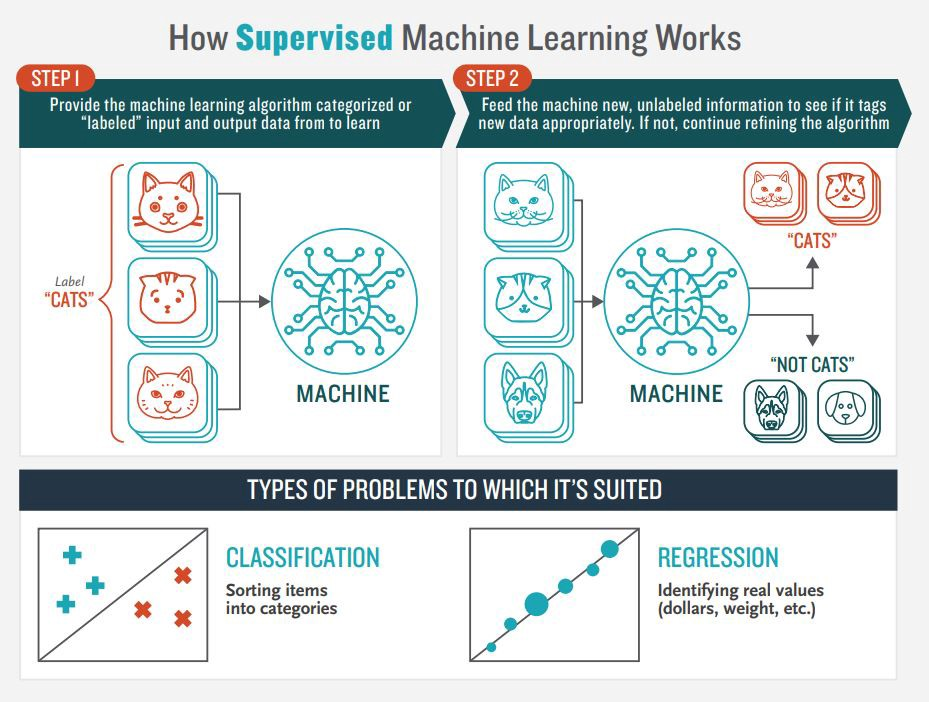
\includegraphics[width=1\textwidth]{figures/1174006/chapter1/supervisedlearning.jpeg}
	\centering
	\caption{Supervised Learning.}
\end{figure}
\noindent
Contoh algoritma yang digunakan pada supervised learning meliputi :
\begin{enumerate}
	\item Clasification (Categorical) and Regression (Numerical)
    \item Logistic Regression
    \item Model Ensemble
	\item Time series
\end{enumerate}

\subsubsection{Klasifikasi}
\hfill\break
Classification adalah tindakan untuk memberikan kelompok pada setiap keadaan. Setiap keadaan berisi sekelompok atribut, salah satunya adalah class attribute. Metode ini butuh untuk menemukan sebuah model yang dapat menjelaskan class attribute itu sebagai fungsi dari input attribute.
\begin{figure}[H]
	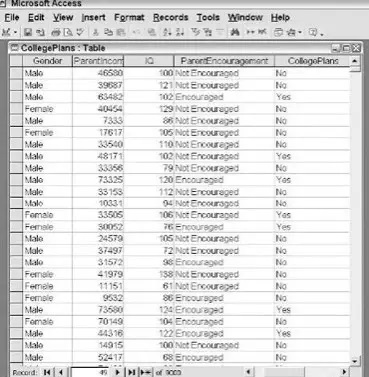
\includegraphics[width=1\textwidth]{figures/1174006/chapter1/clasification.jpg}
	\centering
	\caption{Clasification.}
\end{figure}
\noindent
Class adalah attribute CollegePlans yang berisi dua pernyataan, Yes dan No, perhatikan ini.
\noindent
Sebuah Classification Model akan menggunakan atribut lain dari kasus tersebut (input attribut; yaitu kolom IQ, Gender, ParentIncome, dan ParentEncouragement) untuk dapat menentukan pola (pattern) class (Output Attribute; yaitu Kolom CollegePlans yang berisi Yes atau No).
\noindent
Algoritma Data Mining yang membutuhkan variabel target untuk belajar (sampai mendapatkan rule / pola yang berlaku pada data tersebut) kita standarkan dengan sebuthan dengan Supervised Algorithm.
\noindent
Nah, yang termasuk kepada Classification Algorithm adalah Decision Trees, Neural Network dan Naives Bayes.
\subsubsection{Regresi}
\hfill\break
Metode Regression mirip dengan metode Classification, yang membedakannya adalah metode regression tidak bisa mencari pola yang dijabarkan sebagai class (kelas).
\noindent
Metoda regression bertujuan untuk mecari pola dan menentukan sebuah nilai numerik.
\noindent
Sebuah Teknik Linear Line-fitting sederhana adalah sebuah contoh dari Regression, dimana hasilnya adalah sebuah fungsi untuk menentukan hasil yang berdasarkan nilai dari input.
\noindent
Bentuk yang lebih canggih dari regression sudah mendukung input berupa kategori, jadi tidak hanya input berupa numerik. Teknik paling popular yang digunakan untuk regression adalah linear regression dan logistic regression. Teknik lain yang didukung oleh SQL Server Data mining adalah Regression Trees (bagian dari dari algoritma Microsoft Decission Trees) dan Neural Network.
\noindent
Regression digunakan untuk memecahkan banyak problem bisnis – contohnya untuk memperkirakan metode distribusi, kapasitas distribusi, musim dan untuk memperkirakan kecepatan angin berdasarkan temperatur, tekanan udara, dan kelembaban.
\subsubsection{Unsupervised Learning}
\hfill\break
Unsupervised learning memiliki keunggulan dari supervised learning. Jika supervised learning memiliki label sebagai dasar prediksi baik serta membuat clasification dan regression algorithm memungkinkan. Tetapi dalam realitanya, data real itu banyak yang tidak memiliki label. Label kebanyakan jika data sudah masuk ke ERP apapun bentuk ERPnya dan bagaimana kalo datanya berupa natural input seperti suara, gambar, dan video. Unsupervised learning tidak menggunakan label dalam memprediksi target feautures / variable. Melainkan menggunakan ke samaan dari attribut attribut yang dimiliki. Jika attribut dan sifat-sifat dari data data feature yang diekstrak memiliki kemirip miripan, maka akan dikelompok kelompokan (clustering). Sehingga hal ini akan menimbulkan kelompok kelompok (cluster). Jumlah cluster bisa unlimited. Dari kelompok kelompok itu model melabelkan, dan jika data baru mau di prediksi, maka akan dicocok kan dengan kelompok yang mirip mirip featurenya.
\begin{figure}[H]
	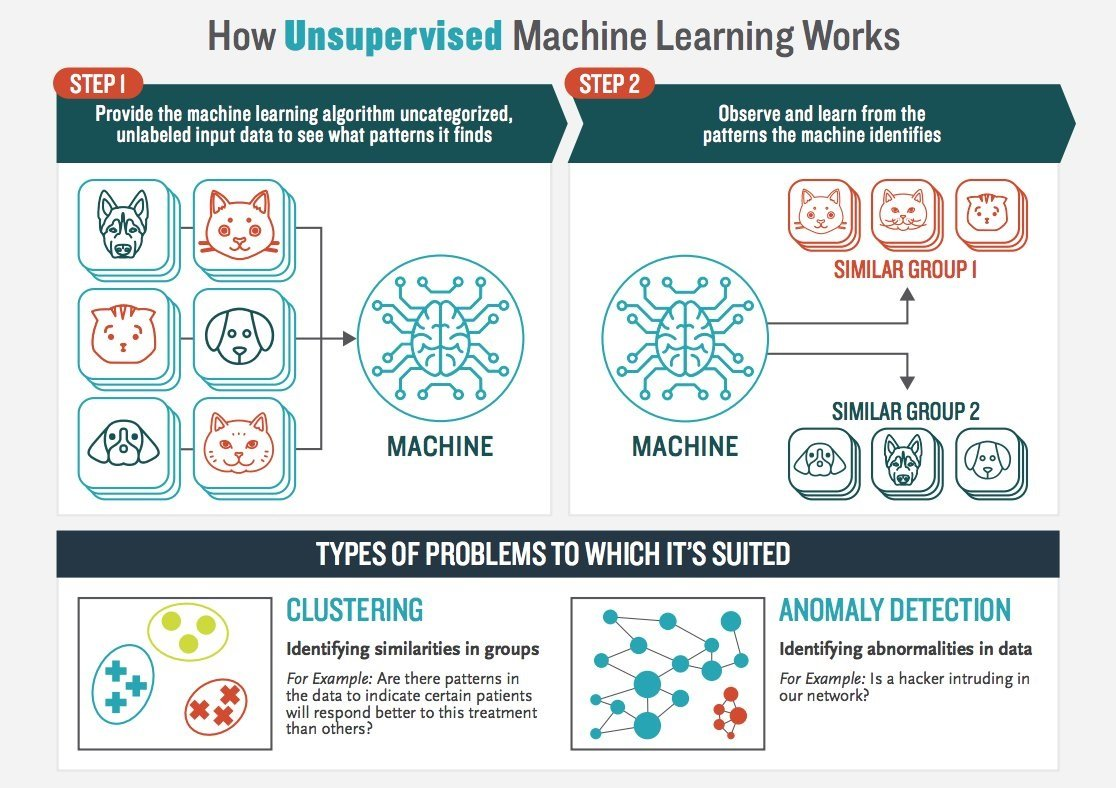
\includegraphics[width=1\textwidth]{figures/1174006/chapter1/unsupervisedlearning.jpg}
	\centering
	\caption{Unsupervised Learning.}
\end{figure}
\noindent
Tetapi unsupervise learning tidak memiliki outcome yang spesifik layaknya di supervise learning, hal ini dikarenakan tidak adanya ground truth / label dasar. Walaupun begitu, unsupervised learning masih dapat memprediksi dari ketidakadaan label dari kemiripan attribute yang dimilik data.
\noindent
Algoritma yang digunakan di unsupervised learning :
\begin{enumerate}
	\item Clustering
    \item Anomaly Detection
    \item Training Model
    \item Association Discovery
\end{enumerate}
\subsubsection{Data Set}
\hfill\break
Dataset adalah objek yang merepresentasikan data dan relasinya di memory. Strukturnya mirip dengan data di database. Dataset berisi koleksi dari datatable dan data relation.
\subsubsection{Training Set}
\hfill\break
Training set adalah bagian dataset yang kita latih untuk membuat prediksi atau menjalankan fungsi dari sebuah algoritma ML lainnya sesuai tujuannya masing-masing. Kita memberikan petunjuk melalui algoritma agar mesin yang kita latih bisa mencari korelasinya sendiri. 
\subsubsection{Testing Set}
\hfill\break
Test set adalah bagian dataset yang kita tes untuk melihat keakuratannya, atau dengan kata lain melihat performanya.
\subsection{Praktek}
\begin{enumerate}
	\item Instalasi  library  scikit  dari  anaconda,  mencoba  kompilasi  dan  uji  coba  ambil contoh kode dan lihat variabel explorer.
	
	\textbf{Instalasi Library Scikit-Learn dengan Anaconda}
	\begin{enumerate}
		\item Pertama pastikan anda telah menginstall Anaconda. Jika sudah menginstall Anaconda, jalankan Anaconda Navigator.
		\begin{figure}[H]
			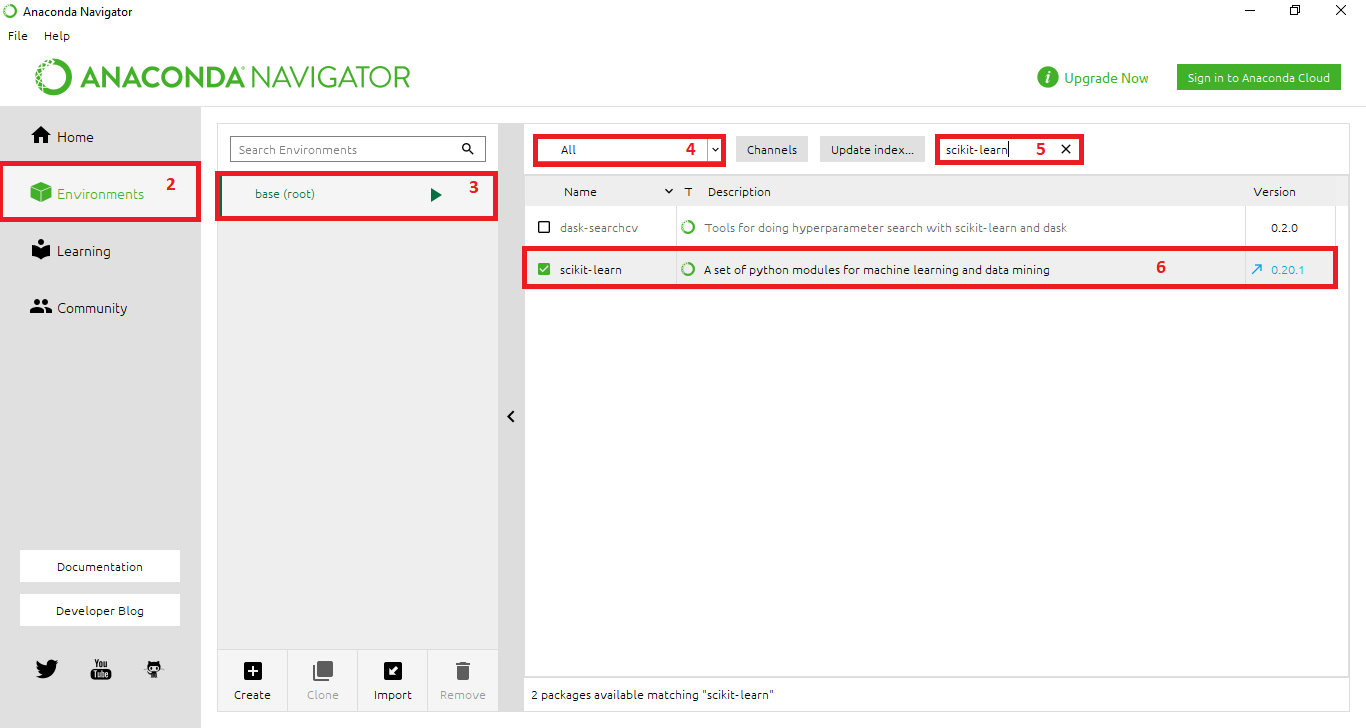
\includegraphics[width=1\textwidth]{figures/1174006/chapter1/praktek/install.png}
			\centering
			\caption{Instalasi Library Scikit-Learn.}
		\end{figure}
		\item Selanjutnya klik menu Environment.
		\item Kemudian klik environment base(root). Disini kita akan melakukan instalasi library scikit- learn di environment base(root).
		\item Lalu pilih All. Untuk menampilkan list library yang ada.
		\item Setelah itu cari scikit-learn di kolom pencarian.
		\item Selanjutnya centang library scikit-learn, lalu klik tombol Apply.
	\end{enumerate}

	\textbf{Mencoba Menggunakan Library scikit-Learn}
	\begin{enumerate}
		\item Pertama jalankan aplikasi Spyder.
		\item Kemudian buat file baru, lalu tambahkan kode berikut.
		\lstinputlisting[language=Python]{src/1174006/chapter1/contoh.py}
		\item Simpan dan jalankan.
		\item Hasil dari variabel explorernya sebagai berikut.
		\begin{figure}[H]
			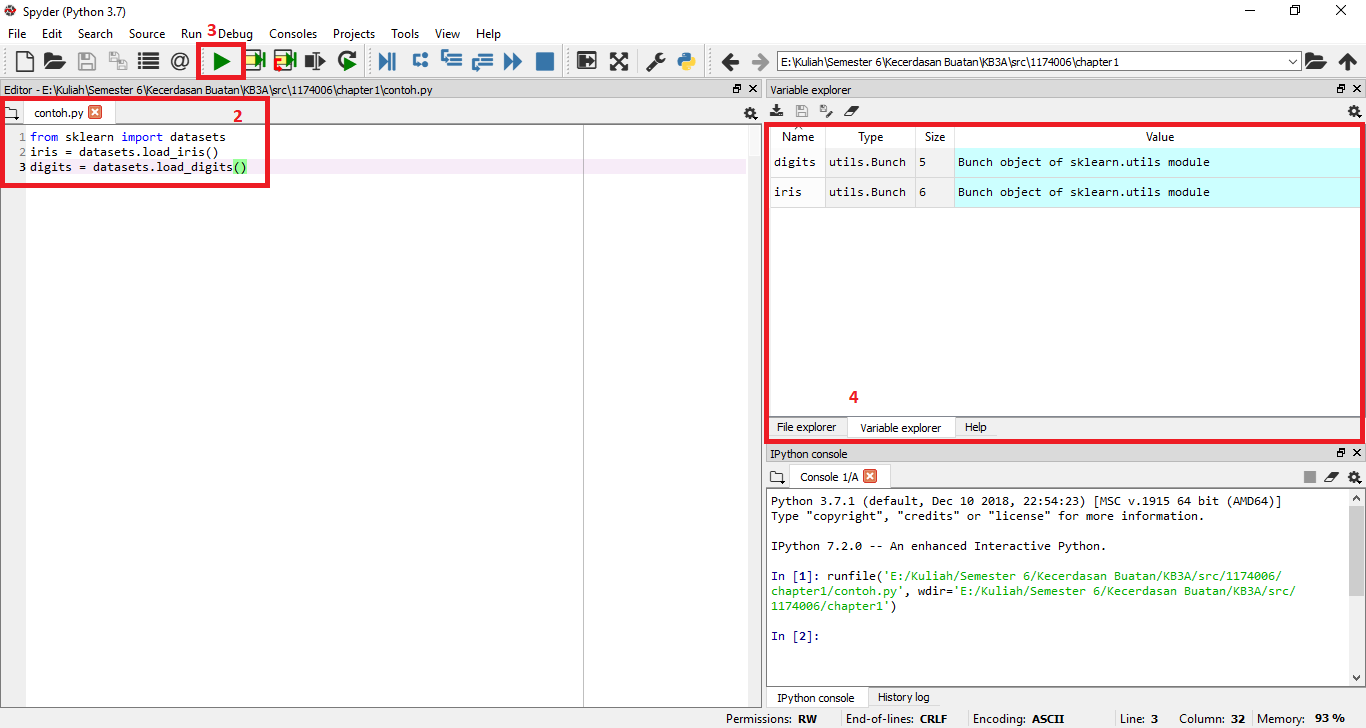
\includegraphics[width=1\textwidth]{figures/1174006/chapter1/praktek/variabel.png}
			\centering
			\caption{Variabel Explorer Library Scikit-Learn.}
		\end{figure}
	\end{enumerate}
	
	\item Mencoba Loading an example dataset, menjelaskan maksud dari tulisan terse-but dan mengartikan per baris.
	\lstinputlisting[language=Python]{src/1174006/chapter1/coba1.py}
	
	Hasilnya akan seperti ini.
	\begin{figure}[H]
		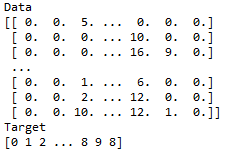
\includegraphics[width=5cm]{figures/1174006/chapter1/praktek/coba1.png}
		\centering
		\caption{Hasil Loading an Example Dataset.}
	\end{figure}

	\item Mencoba  Learning  and  predicting,  menjelaskan  maksud  dari  tulisan  tersebut dan mengartikan per baris.
	\lstinputlisting[language=Python]{src/1174006/chapter1/coba2.py}
	
	Hasilnya akan seperti ini.
	\begin{figure}[H]
		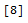
\includegraphics[width=1cm]{figures/1174006/chapter1/praktek/coba2.png}
		\centering
		\caption{Hasil Learning and Predicting.}
	\end{figure}

	\item Mencoba Model persistence, menjelaskan maksud dari tulisan tersebut dan mengartikan per baris.
	\lstinputlisting[language=Python]{src/1174006/chapter1/coba3.py}
	
	Hasilnya akan seperti ini.
	\begin{figure}[H]
		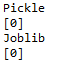
\includegraphics[width=2cm]{figures/1174006/chapter1/praktek/coba3.png}
		\centering
		\caption{Hasil Model Persistence.}
	\end{figure}

	\item Mencoba Conventions, menjelaskan maksud dari tulisan tersebut dan mengartikan per baris.
	\lstinputlisting[language=Python]{src/1174006/chapter1/coba4.py}
	
	Hasilnya akan seperti ini.
	\begin{figure}[H]
		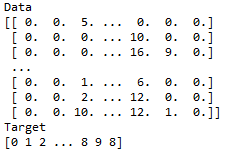
\includegraphics[width=5cm]{figures/1174006/chapter1/praktek/coba1.png}
		\centering
		\caption{Hasil Conventions.}
	\end{figure}

\end{enumerate}

\subsection{Penanganan Error}
\begin{enumerate}
	\item Skrinsut error.
	\begin{itemize}
		\item Name Error
		\hfill\break
		\begin{figure}[H]
			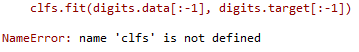
\includegraphics[width=1\textwidth]{figures/1174006/chapter1/error/err3.png}
			\centering
			\caption{Name Error.}
		\end{figure}
		\item Import Error
		\hfill\break
		\begin{figure}[H]
			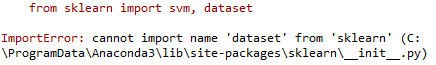
\includegraphics[width=1\textwidth]{figures/1174006/chapter1/error/err1.png}
			\centering
			\caption{Import Error.}
		\end{figure}
		\item Value Error
		\hfill\break
		\begin{figure}[H]
			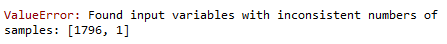
\includegraphics[width=1\textwidth]{figures/1174006/chapter1/error/err2.png}
			\centering
			\caption{Value Error.}
		\end{figure}
		\item Syntax Error
		\hfill\break
		\begin{figure}[H]
			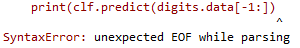
\includegraphics[width=1\textwidth]{figures/1174006/chapter1/error/err4.png}
			\centering
			\caption{Syntax Error.}
		\end{figure}
	\end{itemize}
	\item Tuliskan kode eror dan jenis errornya.
	\begin{itemize}
		\item Name Error
		\hfill\break
		Name Error adalah exception yang terjadi saat syntax melakukan eksekusi terhadap local name atau global name yang tidak terdefinisi.
		\item Import Error
		\hfill\break
		Import Error adalah exception yang terjadi saat syntax melakukan import terhadap library yang tidak terdefinisi.
		\item Value Error
		\hfill\break
		Value Error adalah exception yang terjadi saat syntax memiliki nilai yang tidak valid.
		\item Syntax Error
		\hfill\break
		Syntax Error adalah exception yang terjadi saat ada kesalahan dalam mengetikkan syntax.
	\end{itemize}
	\item Solusi pemecahan masalah error tersebut.
	\begin{itemize}
		\item Name Error
		\hfill\break
		Solusinya adalah memastikan variabel atau function yang dipanggil ada atau tidak salah ketik.
		\item Import Error
		\hfill\break
		Solusinya adalah memastikan library yang dipanggil ada atau tidak salah ketik.
		\item Value Error
		\hfill\break
		Solusinya adalah memastikan nilai yang diinputkan valid.
		\item Syntax Error
		\hfill\break
		Solusinya adalah memastikan syntax yang diketik tidak salah ketik.
	\end{itemize}
\end{enumerate}

\subsection{Bukti Tidak Plagiat}
\begin{figure}[H]
	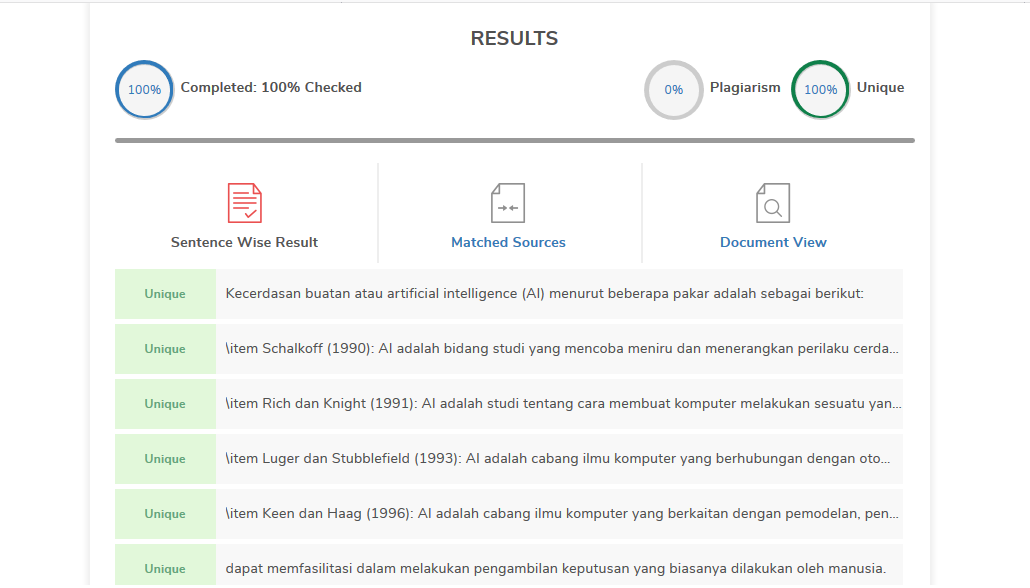
\includegraphics[width=1\textwidth]{figures/1174006/chapter1/plagiat.png}
	\centering
	\caption{Bukti Tidak Plagiat.}
\end{figure}
\section{1174027 - Harun Ar - Rasyid}
\subsection{Teori}
\begin{enumerate}
	\item Sejarah dan Perkembangan
	\hfill\break
	Kecerdasan Buatan atau dalam Bahasa inggris sering disebut Artifical Intelligence yang sering disebut juga sebagai AI, pada 10 tahun lalu masyarakat belum terlalu mengetahui hal tersebut dan masih menjadi bahan candaan dikalangan masyarakat. Awal perkembangan AI dimulai pada tahun 1952-1969 yang dimulai dengan kesuksesan Newwll dan temannya simon menggunakan sebuah program yang disebut dengan General Problem Solver. Program ini dibangun untuk tujuan penyelesaiin masalah secara manusiawi. Pada tahun 1966-1974 perkembangan kecerdasan buatan mulai melambat. Ada 3 faktor utama yang menyebabkan hal itu terjadi:
	\begin{itemize}
		\item Banyak subjek pada program AI yang bermunculan hanya mengandung sedikit atau bahkan sama sekali tidak  mengandung sama sekali pengetahuan (knowledge).
		\item Kecerdasan buatan harus bisa menyelesaikan banyak masalah.
		\item Untuk menghasilkan perilkau intelijensia ada beberapa batasan pada struktur yang bisa digunakan.
	\end{itemize}
	Definisi kecerdasan buatan itu sendiri adalah suatu system teknologi yang didalamnya ditambahakan kecerdasan oleh manusia, kecerdasan buatan diatur dan dikembangkan dalam konteks ilmiah, dan bentukan dari kecerdasan entitas ilmiah yang ada.
	\item Definisi
	\hfill\break
	Supervised learning, klasifikasi, regresi, unsupervised learning, dataset, trainingset dan testingset.
	\begin{itemize}
		\item Supervised Learning
		\hfill\break
		Supervised Learning merupakan sebuah tipe learning yang mempunyai variable input dan variable output, tipe ini juga menggunakan satu algoritma atau lebih dari satu algoritma yang digunakan untuk mempelajari fungsi  pemetaan dari input ke output.
		\item Klasifikasi
		\hfill\break
		Klasifikasi adalah pengelompokan data di mana data yang digunakan memiliki label atau kelas target. Sehingga algoritma untuk menyelesaikan masalah klasifikasi dikategorikan ke dalam pembelajaran terbimbing.
		\item Regresi
		\hfill\break
		regressi metode analisis statistik yang digunakan untuk dapat melihat efek antara dua atau lebih variabel. Hubungan variabel dalam pertanyaan adalah fungsional yang diwujudkan dalam bentuk model matematika. Dalam analisis regresi, variabel dibagi menjadi dua jenis, yaitu variabel respons atau yang biasa disebut variabel dependen dan variabel independen atau dikenal sebagai variabel independen. Ada beberapa jenis analisis regresi, yaitu regresi sederhana yang mencakup linear sederhana dan regresi non-linear sederhana dan regresi berganda yang mencakup banyak linier atau non-linear berganda. Analisis regresi digunakan dalam pembelajaran mesin pembelajaran dengan metode pembelajaran terawasi.
		\item Unsupervised learning 
		\hfill\break
		unsupervised learning jenis pembelajaran di mana kita hanya memiliki data input (input data) tetapi tidak ada variabel output yang terkait. Tujuan dari pembelajaran tanpa pengawasan adalah untuk memodelkan struktur dasar atau distribusi data dengan tujuan mempelajari data lebih lanjut, dengan kata lain, itu adalah fungsi simpulan yang menggambarkan atau menjelaskan data.
		\item Data set
		\hfill\break
		Data set objek yang merepresentasikan data dan relasinya di memory. Strukturnya mirip dengan data di database. Dataset berisi koleksi dari datatable dan datarelation.
		\item Training Set
		\hfill\break
		Training set adalah bagian dari dataset yang di latih untuk membuat prediksi atau menjalankan fungsi dari algoritma ML lain sesuai dengan masing-masing. Memberikan instruksi melalui algoritma sehingga mesin yang di praktikkan dapat menemukan korelasinya sendiri.
		\item Testing Set
		\hfill\break
		testing set adalah bagian dari dataset yang kami uji untuk melihat akurasinya, atau dengan kata lain untuk melihat kinerjanya.
	\end{itemize}
\end{enumerate}
\subsection{Praktek}
\begin{enumerate}
	\item Instalasi Library scikit dari ianaconda, mencoba kompilasi dan uji coba ambil contoh kode dan lihat variabel explorer
	\hfill\break
	\begin{figure}[H]
		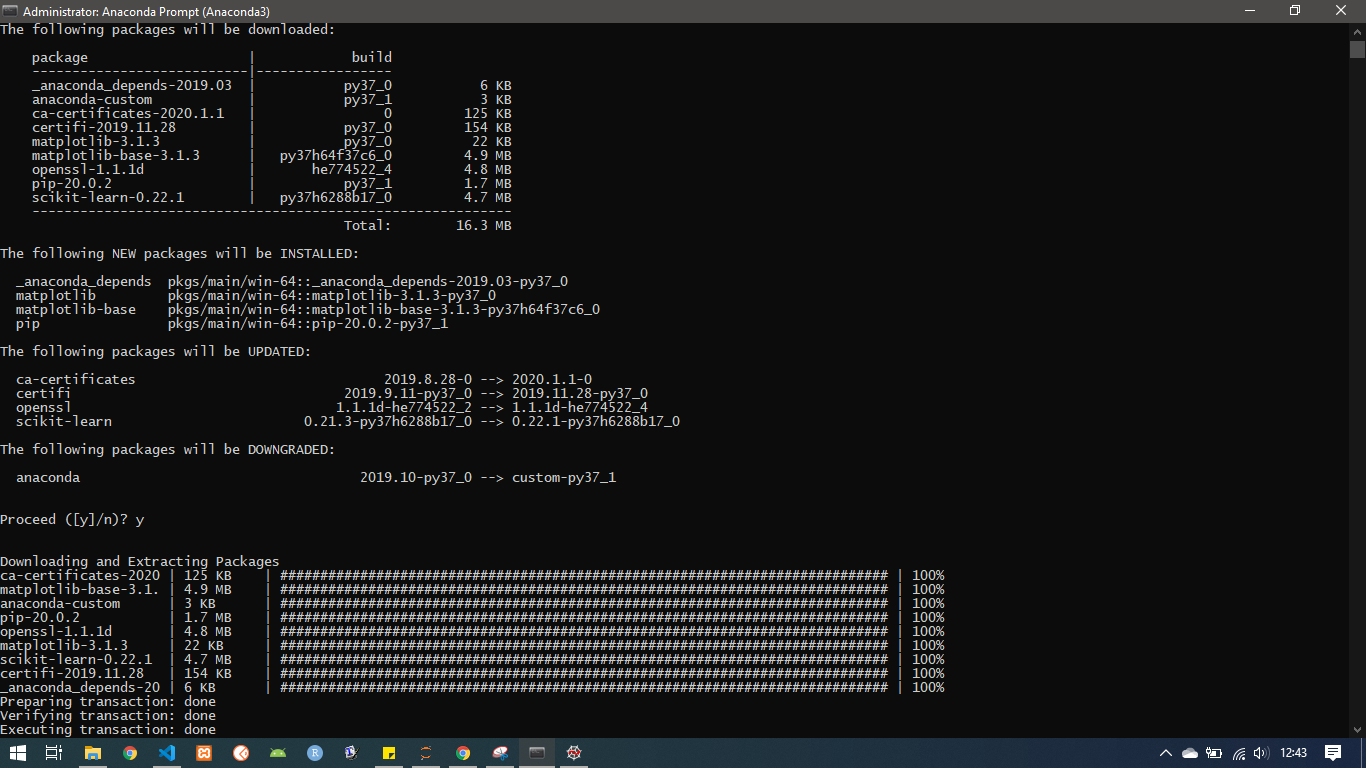
\includegraphics[width=4cm]{figures/1174027/1/instalasi.png}
		\centering
		\caption{Instalasi Package Scikit Learn}
	\end{figure}
	\begin{figure}[H]
		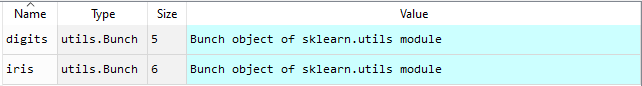
\includegraphics[width=4cm]{figures/1174027/1/variabel.png}
		\centering
		\caption{Isi Variabel Explorer}
	\end{figure}
	\item Mencoba loading an example dataset
	\hfill\break
	\lstinputlisting[firstline=7, lastline=11]{src/1174027/1/1174027.py}
	\item Mencoba Learning dan predicting
	\hfill\break
	\lstinputlisting[firstline=13, lastline=22]{src/1174027/1/1174027.py}
	\item Mencoba Model Persistence
	\hfill\break
	\lstinputlisting[firstline=25, lastline=34]{src/1174027/1/1174027.py}
	\item Mencoba Conventions
	\hfill\break
	\lstinputlisting[firstline=37, lastline=48]{src/1174027/1/1174027.py}
\end{enumerate}
\subsection{Penanganan Error}
\begin{enumerate}
	\item ScreenShoot Error
	\begin{figure}[H]
		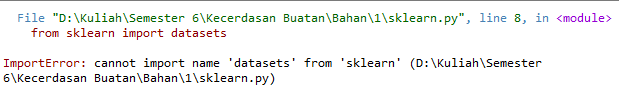
\includegraphics[width=4cm]{figures/1174027/error/1_import.png}
		\centering
		\caption{Import Error}
	\end{figure}
	\begin{figure}[H]
		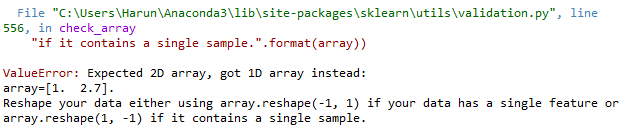
\includegraphics[width=4cm]{figures/1174027/error/1_value.png}
		\centering
		\caption{Value Error}
	\end{figure}
	\item Tuliskan Kode Error dan Jenis Error
	\begin{itemize}
		\item Import Error
		\item Value Error
	\end{itemize}
	\item Cara Penangan Error
	\begin{itemize}
		\item Import Error
		\hfill\break
		Dengan Menginstall Library Yang Tidak Ditemukan
		\item Value Error
		\hfill\break
		Mengubah Bentuk Arraynya, Menjadi 1 Dimensi
	\end{itemize}
\end{enumerate}
\subsection{Bukti Tidak Plagiat}
\begin{figure}[H]
	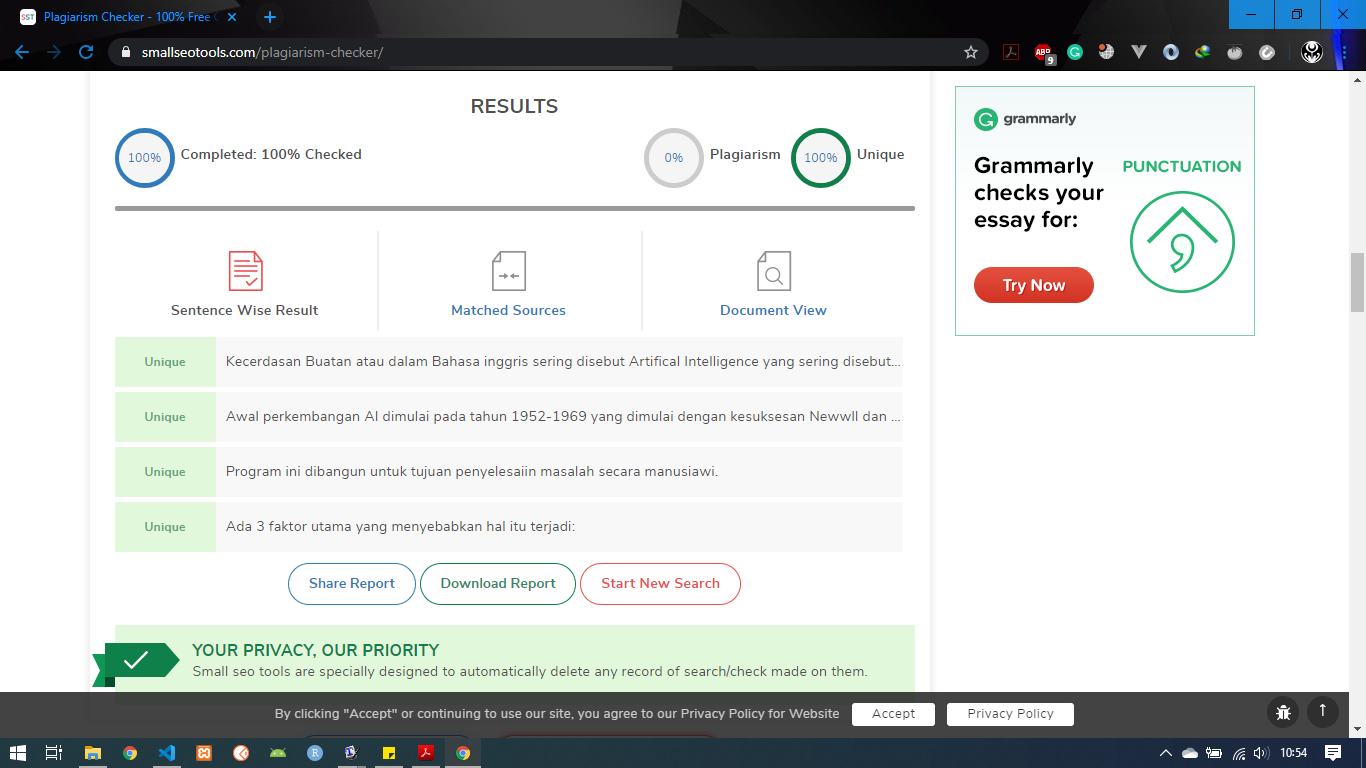
\includegraphics[width=4cm]{figures/1174027/bukti/1.png}
	\centering
	\caption{Bukti Tidak Melakukan Plagiat Chapter 1}
\end{figure}
\section{1174031 - Muhammad Tomy Nur Maulidy}
\subsection{Teori}
\begin{enumerate}
	\item Sejarah dan Perkembangan
	\hfill\break
	Kecerdasan Buatan atau dalam Bahasa inggris sering disebut Artifical Intelligence yang sering disebut juga sebagai AI, pada 10 tahun lalu masyarakat belum terlalu mengetahui hal tersebut dan masih menjadi bahan candaan dikalangan masyarakat. Awal perkembangan AI dimulai pada tahun 1952-1969 yang dimulai dengan kesuksesan Newwll dan temannya simon menggunakan sebuah program yang disebut dengan General Problem Solver. Program ini dibangun untuk tujuan penyelesaiin masalah secara manusiawi. Pada tahun 1966-1974 perkembangan kecerdasan buatan mulai melambat. Ada 3 faktor utama yang menyebabkan hal itu terjadi:
	\begin{itemize}
		\item Banyak subjek pada program AI yang bermunculan hanya mengandung sedikit atau bahkan sama sekali tidak  mengandung sama sekali pengetahuan (knowledge).
		\item Kecerdasan buatan harus bisa menyelesaikan banyak masalah.
		\item Untuk menghasilkan perilkau intelijensia ada beberapa batasan pada struktur yang bisa digunakan.
	\end{itemize}
	Definisi kecerdasan buatan itu sendiri adalah suatu system teknologi yang didalamnya ditambahakan kecerdasan oleh manusia, kecerdasan buatan diatur dan dikembangkan dalam konteks ilmiah, dan bentukan dari kecerdasan entitas ilmiah yang ada.
	\item Definisi
	\hfill\break
	Supervised learning, klasifikasi, regresi, unsupervised learning, dataset, trainingset dan testingset.
	\begin{itemize}
		\item Supervised Learning
		\hfill\break
		Supervised Learning merupakan sebuah tipe learning yang mempunyai variable input dan variable output, tipe ini juga menggunakan satu algoritma atau lebih dari satu algoritma yang digunakan untuk mempelajari fungsi  pemetaan dari input ke output.
		\item Klasifikasi
		\hfill\break
		Klasifikasi adalah pengelompokan data di mana data yang digunakan memiliki label atau kelas target. Sehingga algoritma untuk menyelesaikan masalah klasifikasi dikategorikan ke dalam pembelajaran terbimbing.
		\item Regresi
		\hfill\break
		regressi metode analisis statistik yang digunakan untuk dapat melihat efek antara dua atau lebih variabel. Hubungan variabel dalam pertanyaan adalah fungsional yang diwujudkan dalam bentuk model matematika. Dalam analisis regresi, variabel dibagi menjadi dua jenis, yaitu variabel respons atau yang biasa disebut variabel dependen dan variabel independen atau dikenal sebagai variabel independen. Ada beberapa jenis analisis regresi, yaitu regresi sederhana yang mencakup linear sederhana dan regresi non-linear sederhana dan regresi berganda yang mencakup banyak linier atau non-linear berganda. Analisis regresi digunakan dalam pembelajaran mesin pembelajaran dengan metode pembelajaran terawasi.
		\item Unsupervised learning 
		\hfill\break
		unsupervised learning jenis pembelajaran di mana kita hanya memiliki data input (input data) tetapi tidak ada variabel output yang terkait. Tujuan dari pembelajaran tanpa pengawasan adalah untuk memodelkan struktur dasar atau distribusi data dengan tujuan mempelajari data lebih lanjut, dengan kata lain, itu adalah fungsi simpulan yang menggambarkan atau menjelaskan data.
		\item Data set
		\hfill\break
		Data set objek yang merepresentasikan data dan relasinya di memory. Strukturnya mirip dengan data di database. Dataset berisi koleksi dari datatable dan datarelation.
		\item Training Set
		\hfill\break
		Training set adalah bagian dari dataset yang di latih untuk membuat prediksi atau menjalankan fungsi dari algoritma ML lain sesuai dengan masing-masing. Memberikan instruksi melalui algoritma sehingga mesin yang di praktikkan dapat menemukan korelasinya sendiri.
		\item Testing Set
		\hfill\break
		testing set adalah bagian dari dataset yang kami uji untuk melihat akurasinya, atau dengan kata lain untuk melihat kinerjanya.
	\end{itemize}
\end{enumerate}
\subsection{Praktek}
\begin{enumerate}
	\item Instalasi Library scikit dari ianaconda, mencoba kompilasi dan uji coba ambil contoh kode dan lihat variabel explorer
	\hfill\break
	\begin{figure}[H]
		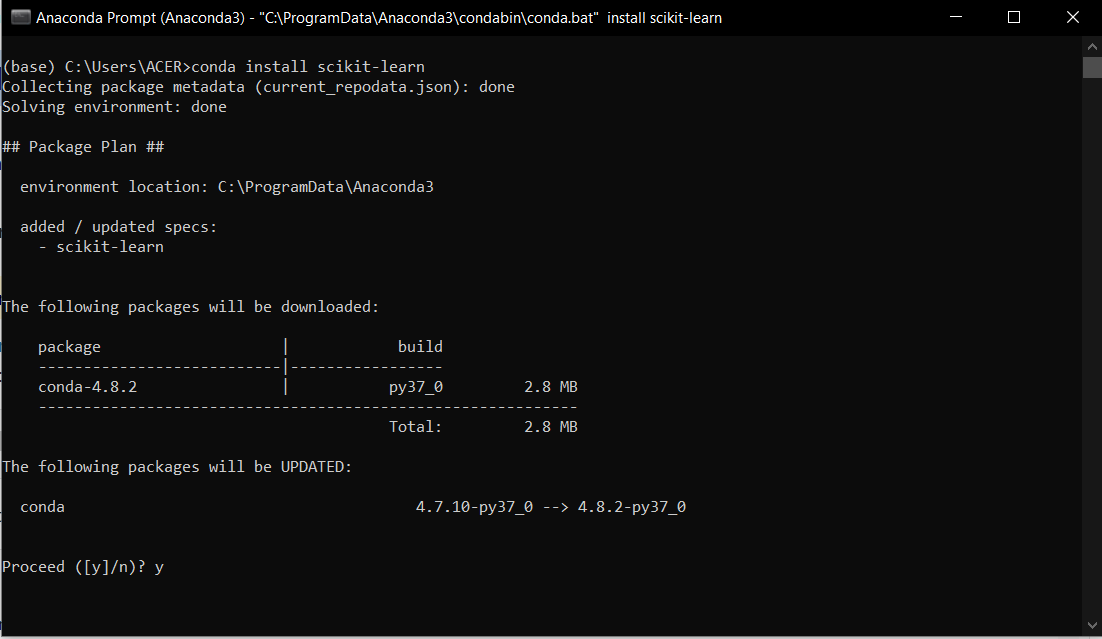
\includegraphics[width=4cm]{figures/1174031/1/1.PNG}
		\centering
		\caption{Instalasi Package Scikit Learn}
	\end{figure}
	\begin{figure}[H]
		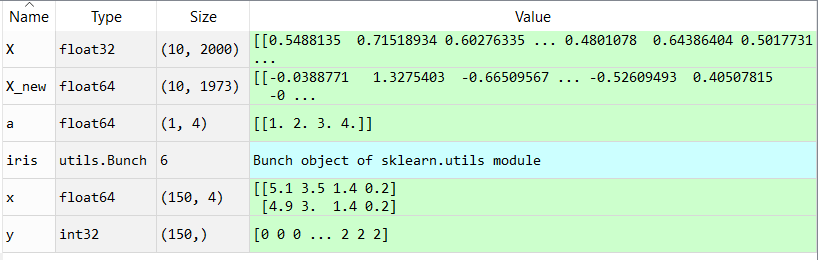
\includegraphics[width=4cm]{figures/1174031/1/2.PNG}
		\centering
		\caption{Isi Variabel Explorer}
	\end{figure}
	\item Mencoba loading an example dataset
	\hfill\break
	\lstinputlisting[firstline=8, lastline=12]{src/1174031/1/1174031.py}
	\item Mencoba Learning dan predicting
	\hfill\break
	\lstinputlisting[firstline=14, lastline=24]{src/1174031/1/1174031.py}
	\item Mencoba Model Persistence
	\hfill\break
	\lstinputlisting[firstline=26, lastline=36]{src/1174031/1/1174031.py}
	\item Mencoba Conventions
	\hfill\break
	\lstinputlisting[firstline=38, lastline=50]{src/1174031/1/1174031.py}
\end{enumerate}
\subsection{Penanganan Error}
\begin{enumerate}
	\item ScreenShoot Error
	\begin{figure}[H]
		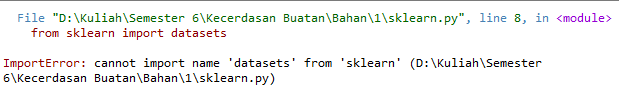
\includegraphics[width=4cm]{figures/1174031/1/error/1.png}
		\centering
		\caption{Import Error}
	\end{figure}
	\begin{figure}[H]
		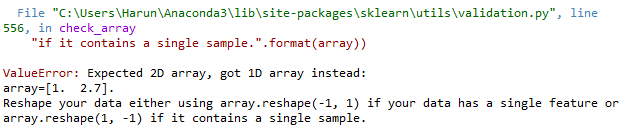
\includegraphics[width=4cm]{figures/1174031/1/error/2.png}
		\centering
		\caption{Value Error}
	\end{figure}
	\item Tuliskan Kode Error dan Jenis Error
	\begin{itemize}
		\item Import Error
		\item Value Error
	\end{itemize}
	\item Cara Penangan Error
	\begin{itemize}
		\item Import Error
		\hfill\break
		Dengan Menginstall Library Yang Tidak Ditemukan
		\item Value Error
		\hfill\break
		Mengubah Bentuk Arraynya, Menjadi 1 Dimensi
	\end{itemize}
\end{enumerate}
\subsection{Bukti Tidak Plagiat}
\begin{figure}[H]
	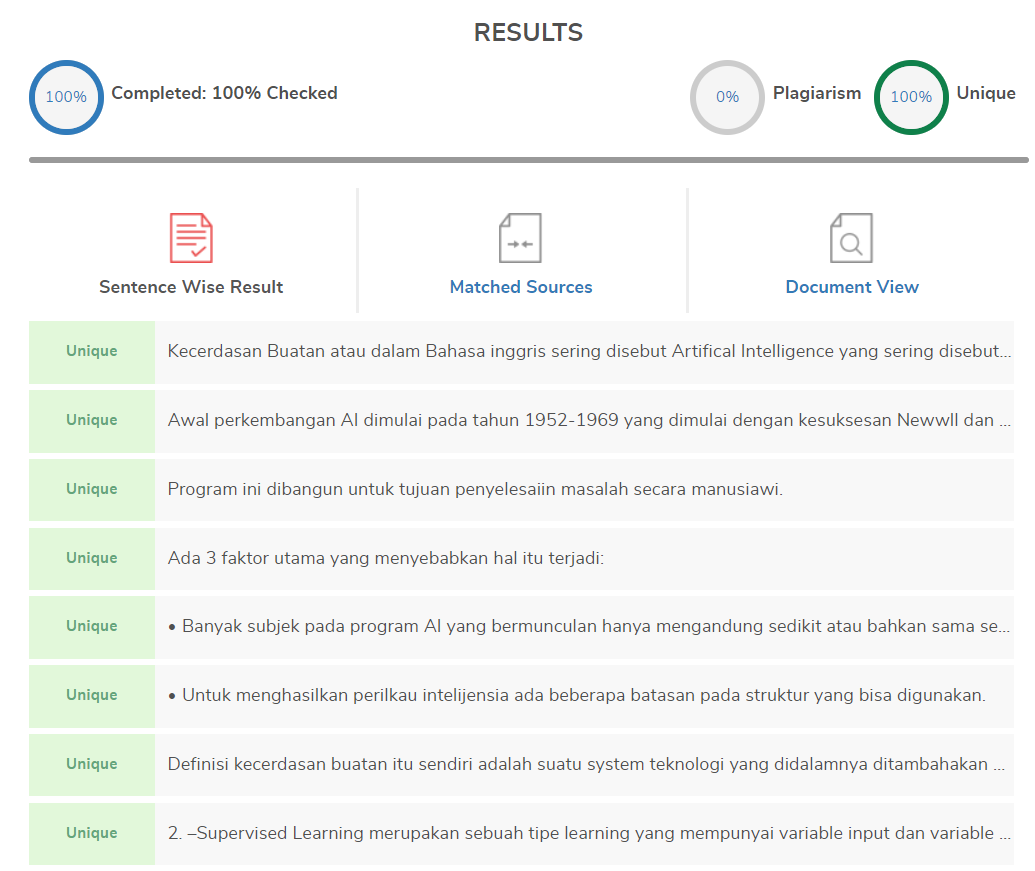
\includegraphics[width=4cm]{figures/1174031/1/plagiat/1.PNG}
	\centering
	\caption{Bukti Tidak Melakukan Plagiat 1}
    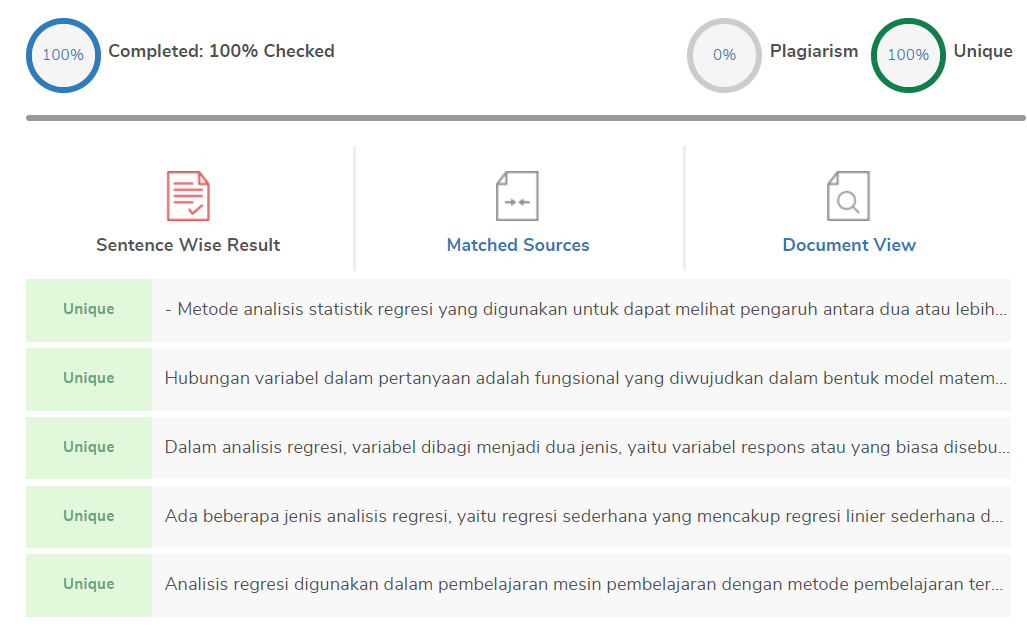
\includegraphics[width=4cm]{figures/1174031/1/plagiat/2.PNG}
	\centering
	\caption{Bukti Tidak Melakukan Plagiat 2}
\end{figure}

\chapter{Chapter 2}
\section{1174006 - Kadek Diva Krishna Murti}
Lorem ipsum dolor sit amet, consectetur adipiscing elit.

\lstinputlisting[firstline=1, lastline=8]{references.bib}
\hfill\break
\begin{figure}[H]
    
\includegraphics[width=4cm]{kreatiflogo.png}
    \centering
    \caption{Kecerdasan Buatan.}
\end{figure}

\begin{enumerate}
	\item Lorem ipsum dolor sit amet, consectetur adipiscing elit.
	\item Lorem ipsum dolor sit amet, consectetur adipiscing elit.
	\item Lorem ipsum dolor sit amet, consectetur adipiscing elit.
\end{enumerate}

\subsection{Teori}

\subsection{Praktek}

\subsection{Penanganan Error}

\subsection{Bukti Tidak Plagiat}
\begin{figure}[H]
	
\includegraphics[width=4cm]{kreatiflogo.png}
	\centering
	\caption{Kecerdasan Buatan.}
\end{figure}
%\section{1174027 - Harun Ar - Rasyid}
\subsection{Teori}
\begin{enumerate}
	\item Jelaskan apa itu binary classication dilengkapi ilustrasi gambar sendiri
	\hfill\break
	\begin{figure}[H]
		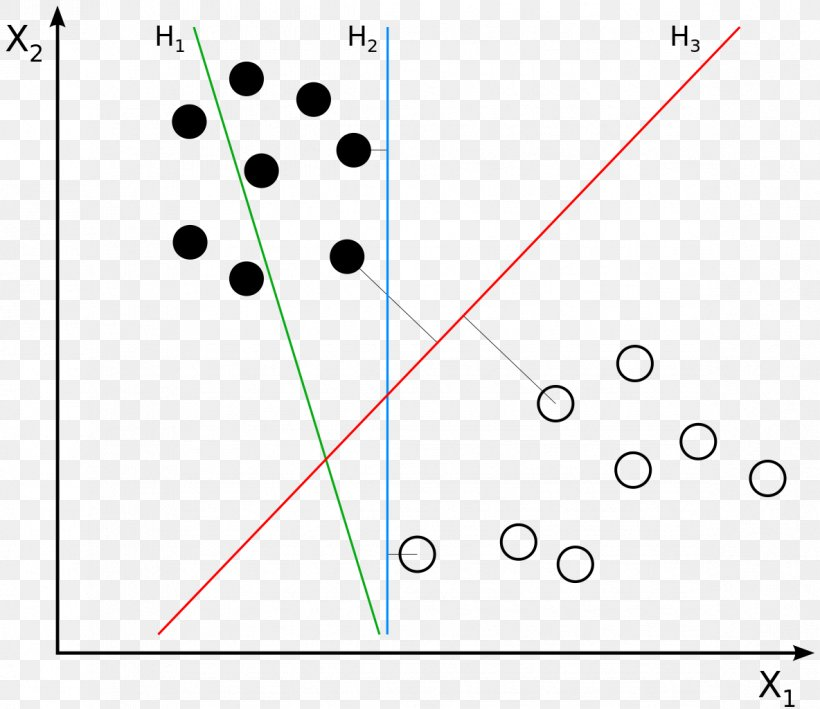
\includegraphics[width=4cm]{figures/1174027/2/1.jpg}
		\centering
		\caption{classication}
	\end{figure}
	Klasifikasi biner atau binomial adalah tugas mengklasifikasikan elemen-elemen dari himpunan yang diberikan ke dalam dua kelompok (memprediksi kelompok mana yang masing-masing dimiliki) berdasarkan aturan klasifikasi. 
	Konteks yang membutuhkan keputusan apakah suatu item memiliki sifat kualitatif atau tidak, beberapa karakteristik tertentu, atau beberapa klasifikasi biner khas meliputi
	\begin{itemize}
		\item Tes medis untuk menentukan apakah pasien memiliki penyakit tertentu atau tidak - properti klasifikasi adalah keberadaan penyakit.
		\item Metode uji "lulus atau gagal" atau kontrol kualitas di pabrik, yaitu memutuskan apakah suatu spesifikasi telah atau belum terpenuhi - klasifikasi Go / no go.
		\item Pengambilan informasi, yaitu memutuskan apakah suatu halaman atau artikel harus dalam hasil pencarian atau tidak - properti klasifikasi adalah relevansi artikel, atau kegunaannya bagi pengguna.
	\end{itemize}
	\hfill\break
	Klasifikasi biner adalah dikotomisasi yang diterapkan untuk tujuan praktis, dan dalam banyak masalah klasifikasi biner praktis, 
	kedua kelompok 2 tidak simetris - daripada akurasi keseluruhan, proporsi relatif dari berbagai jenis kesalahan yang menarik. 
	Misalnya, dalam pengujian medis, false positive (mendeteksi penyakit ketika tidak ada) dianggap berbeda dari false negative 
	(tidak mendeteksi penyakit ketika hadir).
	\item Jelaskan apa itu supervised learning dan unsupervised learning dan clustering dengan ilustrasi gambar sendiri.
	\hfill\break
	\begin{figure}[H]
		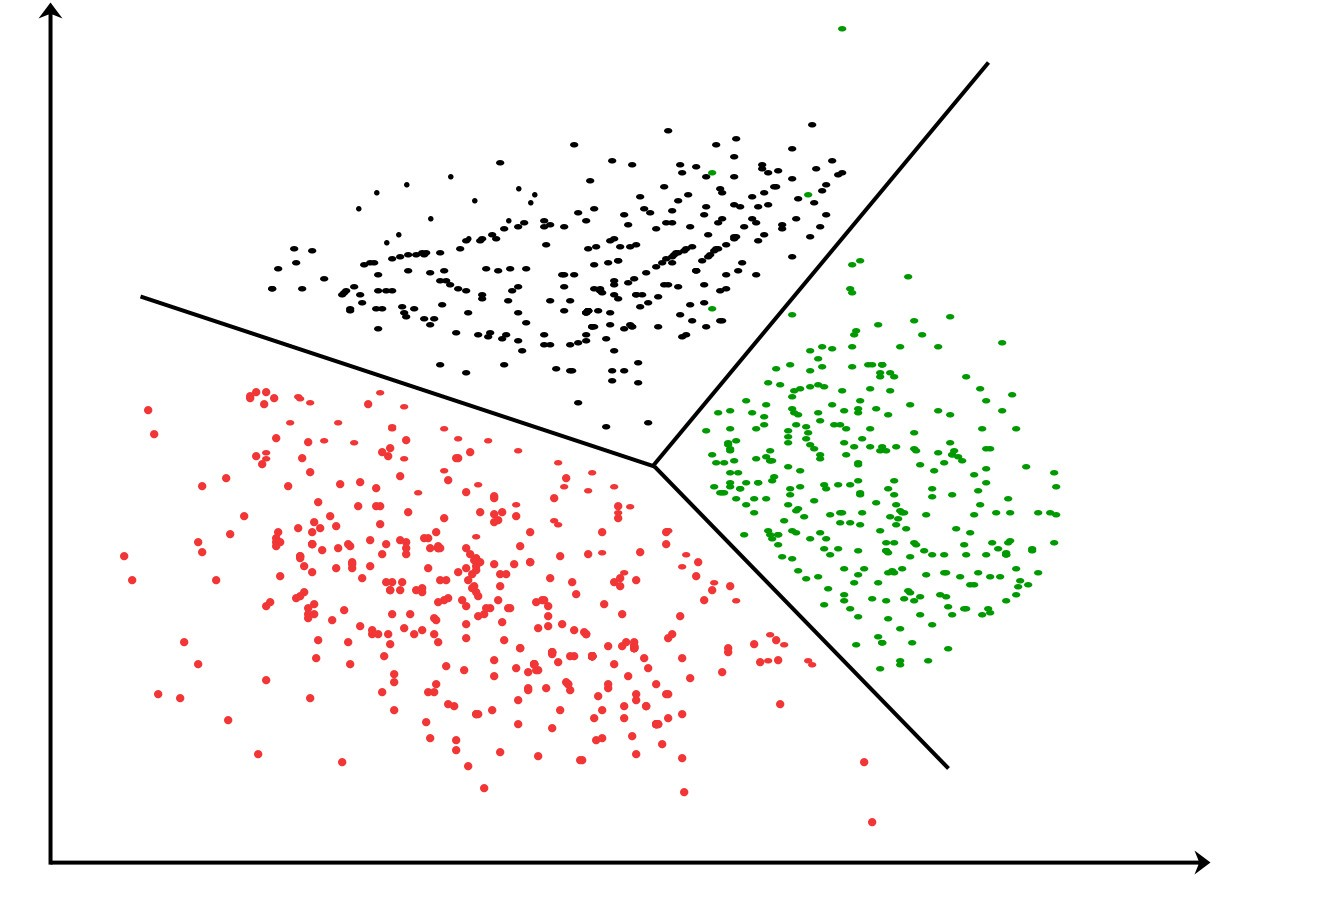
\includegraphics[width=4cm]{figures/1174027/2/clustering.jpg}
		\centering
		\caption{Clustering}
	\end{figure}
	\hfill\break
	Clustering adalah metode menganalisis data, yang sering dikumpulkan sebagai salah satu metode Data Mining, 
	yang dipindahkan adalah mengelompokkan data dengan karakteristik yang sama ke berbagai daerah yang sama dan data dengan karakteristik berbeda ke daerah lain
	\begin{figure}[H]
		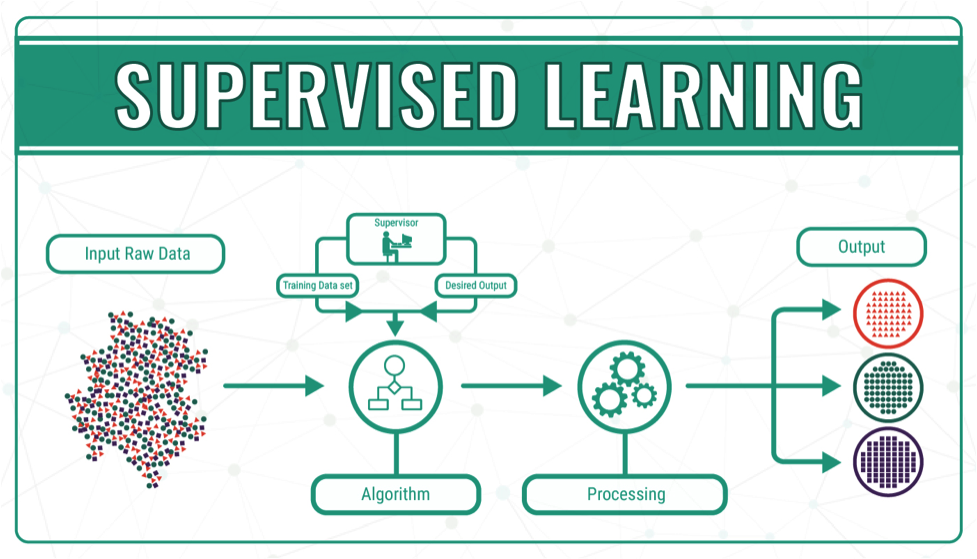
\includegraphics[width=4cm]{figures/1174027/2/supervised.png}
		\centering
		\caption{Supervised Learning}
	\end{figure}
	\hfill\break
	Supervised Learning merupakan sebuah tipe learning yang mempunyai variable input dan variable output, 
	tipe ini juga menggunakan satu algoritma atau lebih dari satu algoritma yang digunakan untuk mempelajari fungsi pemetaan dari input ke output.
	\begin{figure}[H]
		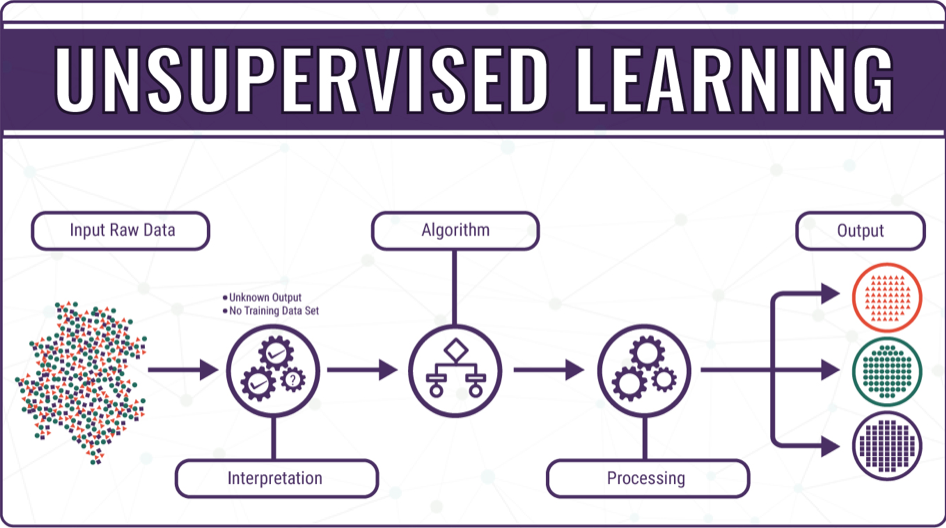
\includegraphics[width=4cm]{figures/1174027/2/unsupervised.png}
		\centering
		\caption{Unsupervised Learning}
	\end{figure}
	\hfill\break
	unsupervised learning jenis pembelajaran di mana kita hanya memiliki data input (input data) tetapi tidak ada variabel output yang terkait. 
	Tujuan dari pembelajaran tanpa pengawasan adalah untuk memodelkan struktur dasar atau distribusi data dengan tujuan mempelajari data lebih lanjut, 
	dengan kata lain, itu adalah fungsi simpulan yang menggambarkan atau menjelaskan data.
	\item Jelaskan apa itu evaluasi dan akurasi dari buku dan disertai ilustrasi contoh dengan gambar sendiri
	\hfill\break
	\begin{figure}[H]
		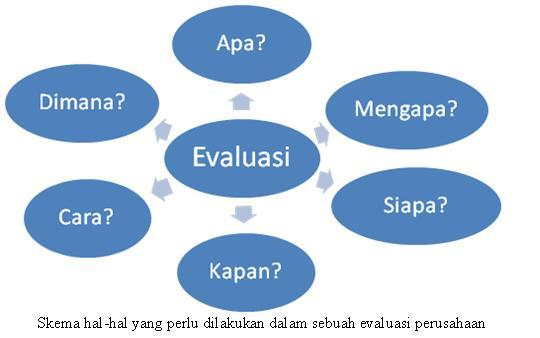
\includegraphics[width=4cm]{figures/1174027/2/Evaluasi.jpg}
		\centering
		\caption{Evaluasi}
	\end{figure}
	\hfill\break
	Evaluasi didefinisikan sebagai penilaian atau penilaian. Nurkancana (1983) menyatakan bahwa evaluasi adalah kegiatan yang dilakukan berkaitan dengan proses 
	penentuan nilai suatu masalah. Sedangkan Raka Joni (1975) menjelaskan evaluasi proses untuk menilai suatu barang, benda atau variasi dengan pertimbangan berbagai 
	faktor yang kemudian disebut Penilaian Nilai.
	\begin{figure}[H]
		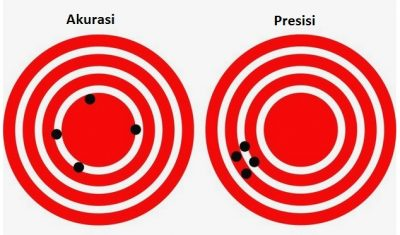
\includegraphics[width=4cm]{figures/1174027/2/akurasi.jpg}
		\centering
		\caption{Akurasi}
	\end{figure}
	\hfill\break
	Akurasi adalah nilai yang dekat dengan nilai aktual. Contohnya mendekati panah target pusat (bullseye).
	\item Jelaskan bagaimana cara membuat dan membaca confusion matrix, buat confusion matrix buatan sendiri.
	\hfill\break
	\begin{figure}[H]
		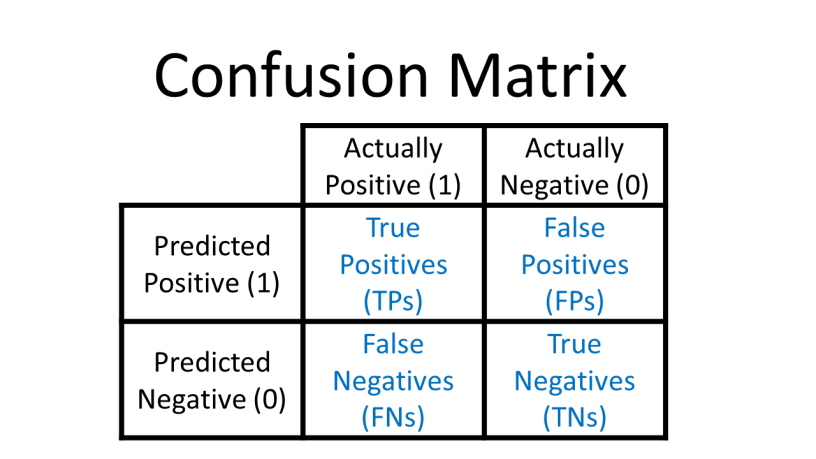
\includegraphics[width=4cm]{figures/1174027/2/confusionmatrix.png}
		\centering
		\caption{Confusionmatrix}
	\end{figure}
	\hfill\break
	\item Jelaskan bagaimana K-fold cross validation bekerja dengan gambar ilustrasi contoh buatan sendiri.
	\hfill\break
	\begin{figure}[H]
		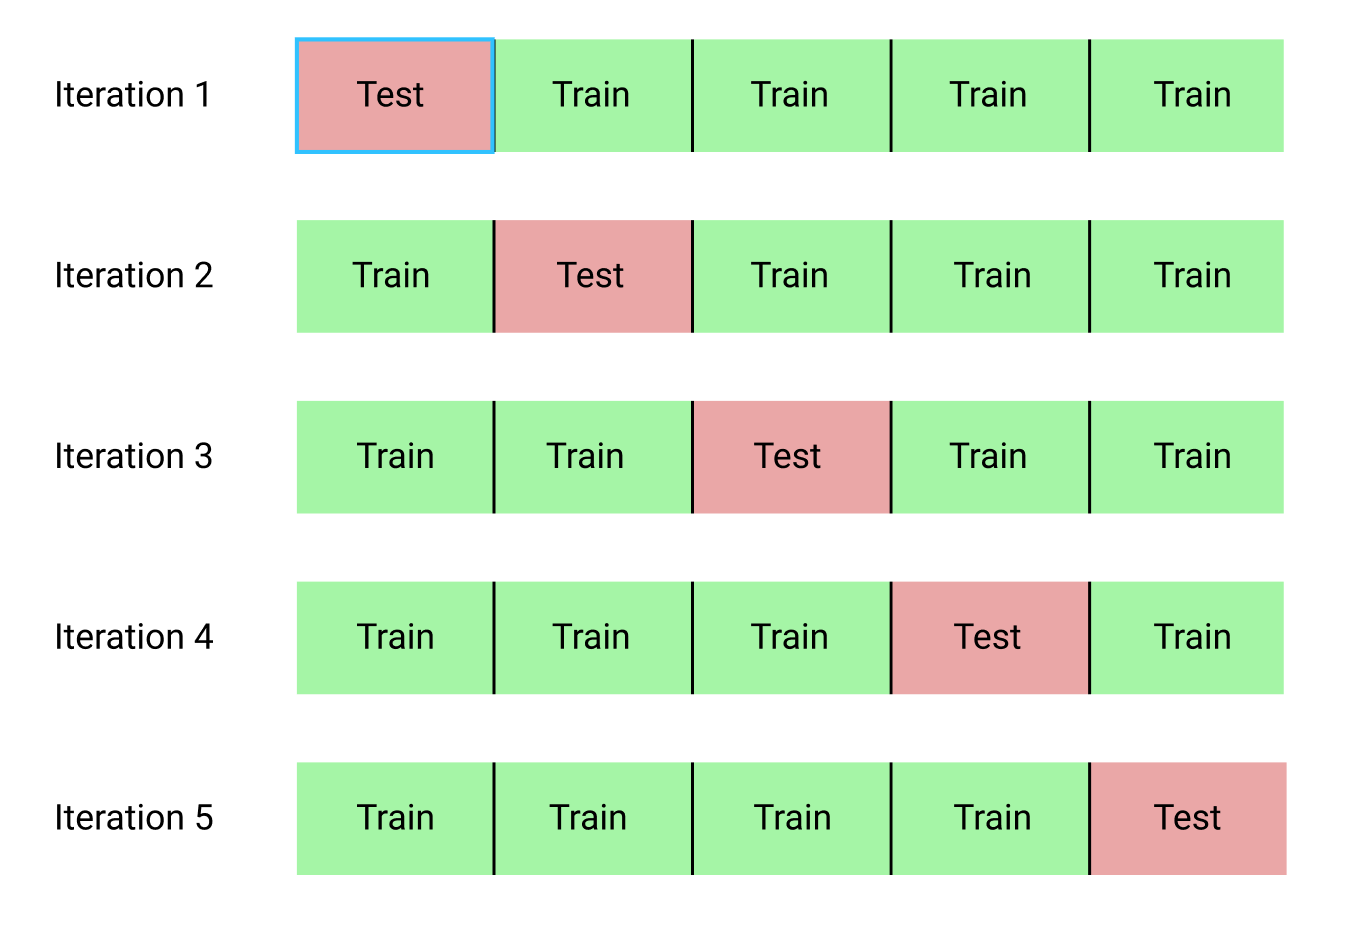
\includegraphics[width=4cm]{figures/1174027/2/kfold.png}
		\centering
		\caption{K-fold}
	\end{figure}
	\hfill\break
	K-fold cross validation adalah salah satu metode untuk mendapatkan kinerja classifier, 
	metode ini dapat digunakan dengan jumlah data yang terbatas (tidak banyak contoh).
	Cara kerja K-fold cross validation adalah sebagai berikut
	\begin{enumerate}
		\item Total instance dibagi menjadi N bagian.
		\item Fold-1 adalah ketika bagian 1 menjadi data uji (data pengujian) dan sisanya menjadi data pelatihan (data pelatihan).
		\hfill\break
		Selanjutnya, hitung keakuratan berdasarkan porsi data. Perhitungan akurasi menggunakan persamaan berikut:
		Akurasi = sigma data uji benar klasifikasi sigma total data uji x 100%%
		\item Fold ke-2 adalah ketika bagian ke-2 menjadi data uji (data pengujian) dan sisanya menjadi data pelatihan (data pelatihan).
		\hfill\break
		Selanjutnya, hitung keakuratan berdasarkan porsi data.4. 
		Demikian seterusnya hingga mencapai fold ke-K. 
		Hitung rata-rata akurasi dari K buah akurasi di atas. 
		Rata-rata akurasi ini menjadi akurasi final.
	\end{enumerate}
	\item Jelaskan apa itu decision tree dengan gambar ilustrasi contoh buatan sendiri.
	\hfill\break
	\begin{figure}[H]
		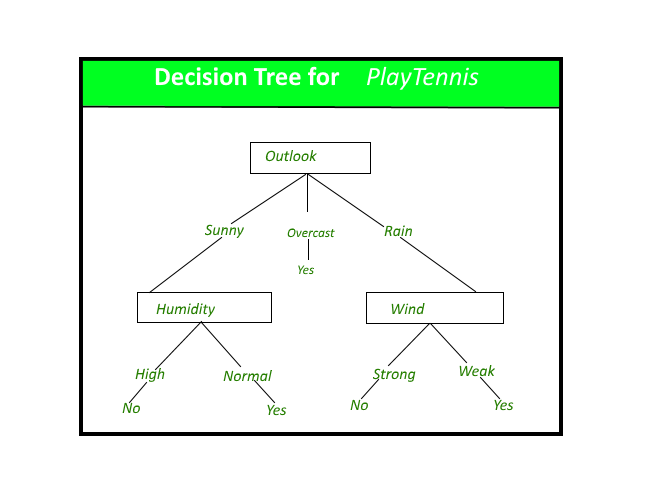
\includegraphics[width=4cm]{figures/1174027/2/Decisiontree.png}
		\centering
		\caption{Decision tree}
	\end{figure}
	\hfill\break
	Pohon keputusan adalah salah satu metode klasifikasi yang paling populer, karena mudah ditafsirkan oleh manusia. 
	Pohon keputusan adalah model prediksi yang menggunakan struktur pohon atau struktur hierarkis.
	Konsep pohon keputusan adalah mengubah data menjadi pohon keputusan dan aturan keputusan. 
	Manfaat utama menggunakan pohon keputusan adalah kemampuannya untuk memecah proses pengambilan keputusan yang menjadi lebih sederhana, 
	sehingga perolehan keputusan akan lebih baik menafsirkan solusi dari masalah.
	\item Jelaskan apa itu information gain dan entropi dengan gambar ilustrasi buatan sendiri
	\hfill\break
	\begin{figure}[H]
		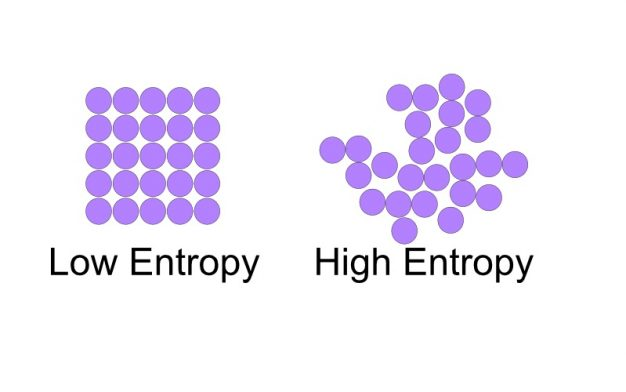
\includegraphics[width=4cm]{figures/1174027/2/entropi.jpg}
		\centering
		\caption{Entropi}
	\end{figure}
	\hfill\break
	Keunggulan informasi adalah kriteria paling populer untuk atribut seleksi. Algoritma C4.5 adalah pengembangan dari algoritma ID3. 
	Karena perkembangan ini, algoritma C4.5 memiliki pekerjaan dasar yang sama dengan algoritma ID3.
	Entropy adalah kuantitas termodinamika yang mengukur energi dalam suatu sistem per unit suhu yang tidak dapat digunakan untuk melakukan bisnis.
\end{enumerate}
\subsection{Praktek}
\lstinputlisting[firstline=1, lastline=80]{src/1174027/2/1174027.py}
\subsection{Penanganan Error}
\begin{enumerate}
	\item SS Error
	\hfill\break
	\begin{figure}[H]
		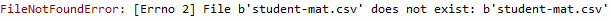
\includegraphics[width=4cm]{figures/1174027/error/2_file_not_found.png}
		\centering
		\caption{File Not Found}
	\end{figure}
	\begin{figure}[H]
		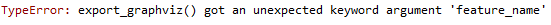
\includegraphics[width=4cm]{figures/1174027/error/2_type.png}
		\centering
		\caption{Type Error FN}
	\end{figure}
	\begin{figure}[H]
		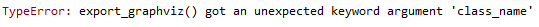
\includegraphics[width=4cm]{figures/1174027/error/2_type2.png}
		\centering
		\caption{Type Error Class name}
	\end{figure}
	\begin{figure}[H]
		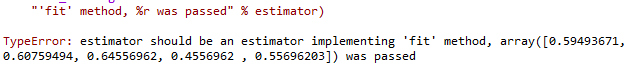
\includegraphics[width=4cm]{figures/1174027/error/2_type3.png}
		\centering
		\caption{Type Error}
	\end{figure}
	\begin{figure}[H]
		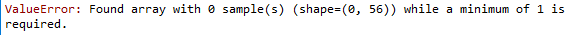
\includegraphics[width=4cm]{figures/1174027/error/2_value.png}
		\centering
		\caption{Value Error}
	\end{figure}
	\item Tuliskan kode error dan jenis errornya
	\hfill\break
	\begin{itemize}
		\item File Not Found
		\item Type Error
		\item Value Error
	\end{itemize}
	\item Solusi pemecahan masalah error
	\hfill\break
	\begin{itemize}
		\item File Not Found
		\hfill\break
		Dengan Cara Mengecek file tersebut apakah berada pada directory yang sama, kemudian run all
		\item Type Error
		\hfill\break
		Dengan cara cek kembali baris code yang bermasalah, dan run setiap sectionya
		\item Value Error
		\hfill\break
		Mendownload kembali datanya dari tahun 1962
	\end{itemize}
\end{enumerate}
\subsection{Bukti Tidak Plagiat}
\begin{figure}[H]
	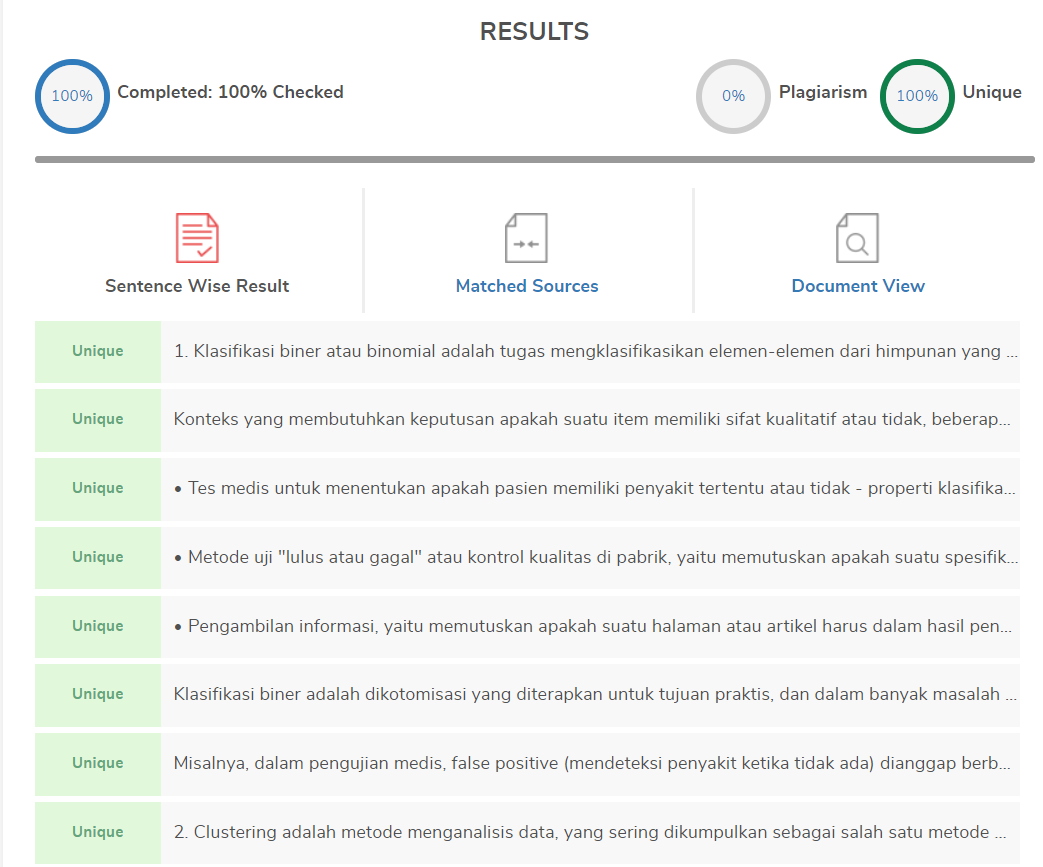
\includegraphics[width=4cm]{figures/1174027/bukti/2.png}
	\centering
	\caption{Bukti Tidak Melakukan Plagiat Chapter 2}
\end{figure}

\chapter{Chapter 3}
\section{1174006 - Kadek Diva Krishna Murti}
Lorem ipsum dolor sit amet, consectetur adipiscing elit.

\lstinputlisting[firstline=1, lastline=8]{references.bib}
\hfill\break
\begin{figure}[H]
    
\includegraphics[width=4cm]{kreatiflogo.png}
    \centering
    \caption{Kecerdasan Buatan.}
\end{figure}

\begin{enumerate}
	\item Lorem ipsum dolor sit amet, consectetur adipiscing elit.
	\item Lorem ipsum dolor sit amet, consectetur adipiscing elit.
	\item Lorem ipsum dolor sit amet, consectetur adipiscing elit.
\end{enumerate}

\subsection{Teori}

\subsection{Praktek}

\subsection{Penanganan Error}

\subsection{Bukti Tidak Plagiat}
\begin{figure}[H]
	
\includegraphics[width=4cm]{kreatiflogo.png}
	\centering
	\caption{Kecerdasan Buatan.}
\end{figure}
%\section{1174027 - Harun Ar - Rasyid}
\subsection{Teori}
\begin{enumerate}
	\item Jelaskan apa itu random forest, sertakan gambar ilustrasi buatan sendiri.
	\hfill\break
	Random Forest merupakan algoritma yang digunakan terhadapap klasifikasi data dalam jumlah yang besar. Klasifikasi pada random forest dilakukan dengan penggabungan dicision tree dengan melakuakn training terhadap sempel data yang dimiliki. Semakin banyak dicision tree maka data yang di dapat akan semakin akurat. Untuk gambar Random Forest dapat dilihat dibawah ini :
	\begin{figure}[H]
	\centering
		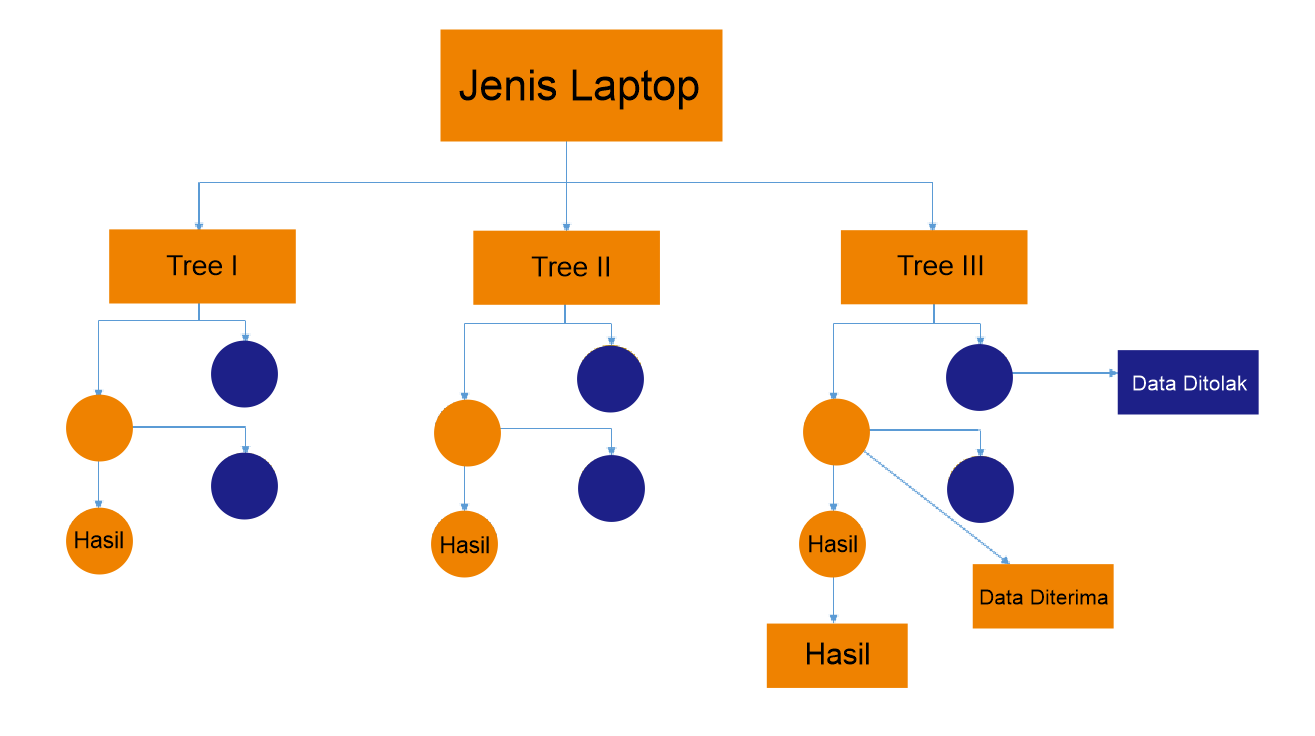
\includegraphics[width=4cm]{figures/1174027/3/1.png}
		\caption{Random Forest.}
	\end{figure}
	\item Jelaskan cara membaca dataset kasus dan artikan makna setiap file dan isi field masing-masing file.
	\hfill\break
	\begin{itemize}
		\item Pertama download dataset terlebih dahulu lalu buka dengan menggunakan software spyder guna melihat isi dari dataset tersebut.
		\item Data tersebut memiliki extensi file bernama .txt dan didalamnya terdapat class dari field.
		\item Misalnya saja pada data jenis burung memiliki file index dan angka, dimana index berisi angka yang memiliki makna berupa jenis burung.
		\item bahkan nama burung sedangkan field memiliki isi nilai berupa 0 dan 1 yang dimana sifatnya boolean atau Ya dan Tidak.
		\item Hal ini dikarenakan komputer hanya dapat membaca bilangan biner maka dari itu field yang di isikan berupa angka.
		\item Artinya angka 0 berarti tidak dan angka 1 berarti Ya.
	\end{itemize}
	\item Jelaskan apa itu cross validation.
	\hfill\break
	Cross Validation merupakan sebuah teknik validasi model yang berfungsi untuk melakukan penilaian bagaimana hasil analisis statistik akan digeneralisasi ke data yang lebih independen. Cross validation digunakan dengan tujuan prediksi, dan bila kita ingin memperkirakan seberapa akurat model model prediksi yang dilakukan dalam sebuah praktek. Tujuan dari cross validation yaitu untuk mendefinisikan dataset guna menguju dalam fase pelatihan untuk membatasi masalah seperti overfitting dan underfitting serta mendapatkan wawasan tentang bagaimana model akan digeneralisasikan ke set data independen.
	\item Jelaskan apa arti score 44 \% pada random forest, 27\% pada decission tree dan 29 \% dari SVM.
	\hfill\break
	Dimana Score 44 \% diperoleh dari hasil pengelohan dataset jenis burung. Dimana akan dilakukan proses pembagian data testing dan data training lalu diproses dan menghasilkan score sebanyak 44 \% dimana menjelaskan bahwa score tersebut digunakan sebagai pembanding dalam tingkat keakuratannya. Pada dicision tree akan memperoleh data lebih kecil yaitu sebanyak 27 \% hal ini dikarenakan data yang diolah menggunakan dicision tree dibagi menjadi beberapa tree dan lalu disimpulkan untuk mendapatkan data yang akurat. Pada SVM akan memperoleh score sebanyak 29 \% hal ini dikarenakan data yang dimiliki masih bernilai netral sehingga tingkat keakuratannya masih belum jelas.
	\item Jelaskan bagaimana cara membaca confusion matriks dan contohnya memakai gambar atau ilustrasi sendiri.
	\hfill\break
	Untuk membaca confusion matriks dapat menggunakan source code sebagai berikut :
	\lstinputlisting[firstline=233, lastline=237]{src/1174027/3/1174027_teori.py}
	\hfill\break
	Dimana numpy akan mengurus semua data yang berhubungan dengan matrix. Pada source code tersebut digunakan dalam melakukan read pada dataset burung dengan menggunakan metode confusion matrix. Dalam confusion matrix memiliki 4 istilah yaitu True Positive yang merupakan data posotif yang terditeksi benar, True Negatif yang merupakan data negatif akan tetapi terditeksi benar, False Positif merupakan data negatif namun terditeksi sebagai data positif, False Negatif merupakan data posotif namun terditeksi sebagai data negatif. Adapun contoh hasil read dataset menggunakan confusion matrix dapat dilihat dibawah ini :
	\begin{figure}[H]
	\centering
		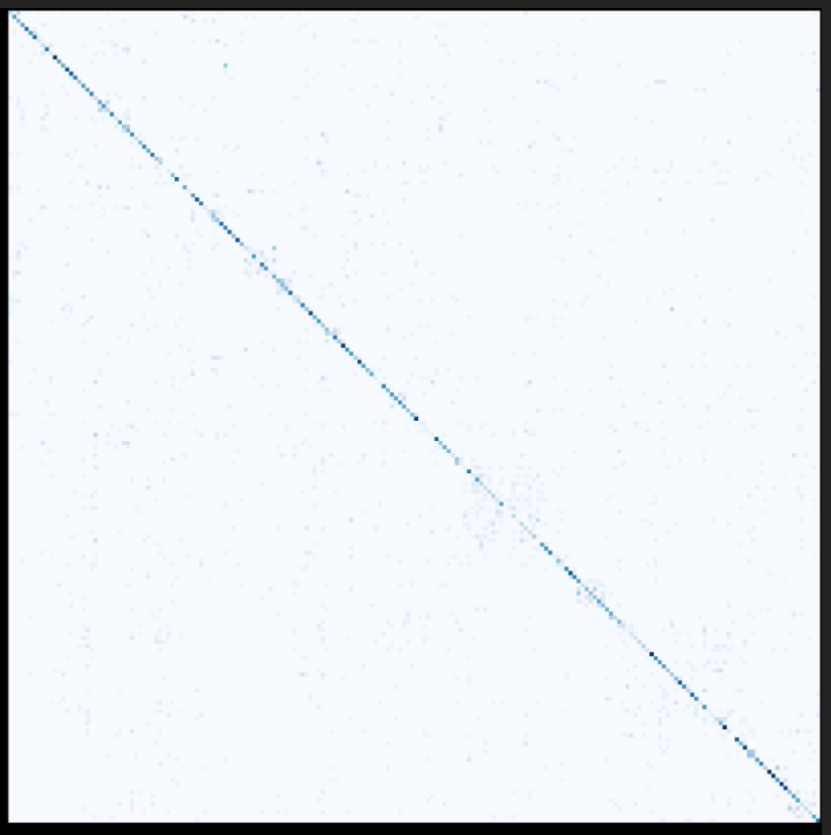
\includegraphics[width=2cm]{figures/1174027/3/2.png}
		\caption{Confusion Matriks.}
	\end{figure}
	\item Jelaskan apa itu voting pada random forest disertai dengan ilustrasi gambar sendiri
	\hfill\break
	Voting pada random forest ialah sebuah proses pemilihan dari tree yang dimana akan dimunculkan hasilnya dan disimpulkan menjadi informasi yang pasti. Untuk lebih jelasnya saya akan memberikan sebuah contoh bagaimana voting bekerja : 
	\begin{figure}[H]
	\centering
		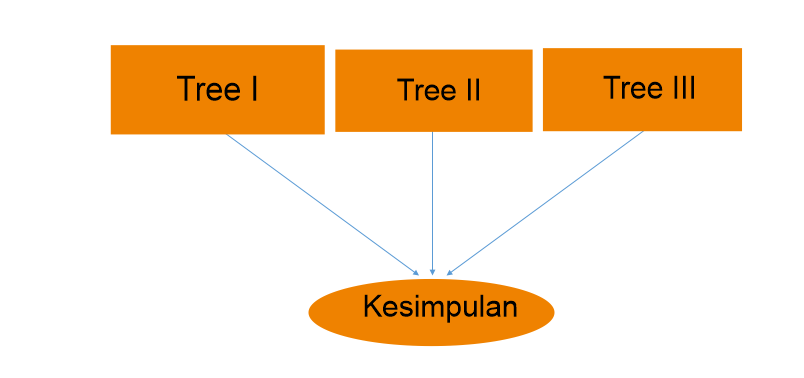
\includegraphics[width=4cm]{figures/1174027/3/3.png}
		\caption{Decision Tree.}
	\end{figure}
	Dimana ditunjukkan pada gambar diatas terdapat 3 tree. Dalam tree tersebut akan dilakukan proses voting. Saya akan memberikan contoh kasus, dimana akan diadakan voting untuk menentukan sebuah laptop. Dalam tree akan diberikan sejumlah data misalnya saja data tersebut berupa gambar, yang dimana data tersebut akan dipilih dengan cara voting. Hasil voting akhir dari setiap tree menunjukkan laptop asus, yang berarti kesimpulan dari data yang telah diberikan menyatakan gambar tersebut adalah laptop asus. Bagaimana apabila terjadi perbedaan data misalnya saja pada tree 1 dan 2 menunyatakan laptop asus sedangkan pada tree 3 menyatakan laptop HP, maka kesimpulan yang di ambil adalah laptop asus dikarenakan hasil voting terbanyak adalah laptop asus.
\end{enumerate}
\subsection{Praktek}
\begin{enumerate}
	\item Buat aplikasi sederhana menggunakan pandas dan jelaskan arti setiap baris kode yang dibuat(harus beda dengan teman sekelas).
	\hfill\break
	\lstinputlisting[firstline=9, lastline=12]{src/1174027/3/1174027_praktek.py}
	Kode di atas digunakan untuk mengimpor atau mengirim library pandas sebagai pd, Hasilnya adalah sebagai berikut :
	\begin{figure}[H]
	\centering
		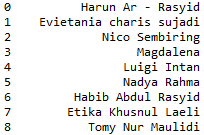
\includegraphics[width=4cm]{figures/1174027/3/hasil1.png}
		\caption{Hasil Soal 1.}
	\end{figure}
	\item buat aplikasi sederhana menggunakan numpy dan jelaskan arti dari setiap baris kode yang dibuat(harus beda dengan teman sekelas)
	\hfill\break
	\lstinputlisting[firstline=14, lastline=16]{src/1174027/3/1174027_praktek.py}
	Fungsi sum disini berguna untuk menjumlahkan data. Hasilnya adalah sebagai berikut :
	\begin{figure}[H]
	\centering
		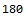
\includegraphics[width=4cm]{figures/1174027/3/hasil2.png}
		\caption{Hasil Soal 2.}
	\end{figure}
	\item buat aplikasi sederhana menggunakan matplotlib dan jelaskan arti dari setiap baris kode(harus beda dengan teman sekelas)
	\hfill\break
	\lstinputlisting[firstline=18, lastline=23]{src/1174027/3/1174027_praktek.py}
	Jalankan source code diatas dengan spyder atau anaconda sehingga hasilnya akan seperti berikut : 
	\begin{figure}[H]
	\centering
		\includegraphics[width=4cm]{figures/1174027/3/hasil3.png}
		\caption{Hasil Soal 3.}
	\end{figure}
	\item jalankan program klasifikasi Random Forest pada bagian teori bab ini. Tunjukkan keluarannya dari komputer sendiri dan artikan maksud setiap luaran yang didapatkan.
	\hfill\break
	\begin{itemize}
		\item Source Code pertama pada random forest berfungsi untuk membaca dataset yang memiliki format text file dengan mendefinisikan variabel yang bernama imgatt. Variabel tersebut berisi value untuk membaca data. 
		\lstinputlisting[firstline=10, lastline=14]{src/1174027/3/1174027_teori.py}
		\item Pada source code berikutnya akan mengembalikan baris teratas dari DataFrame variabel imgatt.
		\lstinputlisting[firstline=19, lastline=19]{src/1174027/3/1174027_teori.py}
		\item Pada output berikutnya akan menampilkan jumlah kolom dan baris dari DataFrame imgatt. 
		\lstinputlisting[firstline=24, lastline=24]{src/1174027/3/1174027_teori.py}
		\item Variabel imgatt2 telah menggunakan function yang bernama pivot guna mengubah kolom jadi baris dan sebaliknya dari DataFrame sebelumnya.
		\lstinputlisting[firstline=29, lastline=29]{src/1174027/3/1174027_teori.py}
		\item Variabel imgatt2 head berfungsi untuk mengembalikan value teratas pada DataFrame imgatt2.
		\lstinputlisting[firstline=34, lastline=34]{src/1174027/3/1174027_teori.py}
		\item Menghasilkan jumlah kolom dan baris pada DataFrame imgatt2.
		\lstinputlisting[firstline=39, lastline=39]{src/1174027/3/1174027_teori.py}
		\item Menunjukkan dalam melakukan pivot yang mana imgid menjadi sebuah index yang unik.
		\lstinputlisting[firstline=44, lastline=47]{src/1174027/3/1174027_teori.py}
		\item Akan melakukan load jawabannya yang berisi apakah burung tersebut termasuk spesies yang mana. Kolom tersebut yaitu imgid dan label.
		\lstinputlisting[firstline=52, lastline=52]{src/1174027/3/1174027_teori.py}
		\item Menunjukkan bahwa jumlah baris sebanyak 11788 dan kolom 1 yang dimana kolom tersebut adalah jenis spesies pada burung.
		\lstinputlisting[firstline=57, lastline=57]{src/1174027/3/1174027_teori.py}
		\item Melakukan join antara imgatt2 dengan imglabels dikarenakan memiliki isi yang sama sehingga akan mendapatkan sebuah data ciri-ciri dan data jawaban sehingga bisa dikategorikan sebagai supervised learning.
		\lstinputlisting[firstline=62, lastline=63]{src/1174027/3/1174027_teori.py}
		\item Melakukan drop pada label yang ada didepan dan akan menggunakan label yang baru di joinkan.
		\lstinputlisting[firstline=68, lastline=69]{src/1174027/3/1174027_teori.py}
		\item Mengecek isi 5 data teratas pada df att.
		\lstinputlisting[firstline=74, lastline=74]{src/1174027/3/1174027_teori.py}
		\item Mengecek isi data teratas dari df label.
		\lstinputlisting[firstline=79, lastline=79]{src/1174027/3/1174027_teori.py}
		\item Membagi 8000 row pertama menjadi data training dan sisanya adalah data testing.
		\lstinputlisting[firstline=84, lastline=90]{src/1174027/3/1174027_teori.py}
		\item Pemanggilan class RandomForestClassifier. Dimana artinya menunjukkan banyak kolom pada setiap tree adalah 50.
		\lstinputlisting[firstline=95, lastline=96]{src/1174027/3/1174027_teori.py}
		\item Menunjukkan hasil prediksi dari Random Forest.
		\lstinputlisting[firstline=101, lastline=101]{src/1174027/3/1174027_teori.py}
		\item Menampilkan besaran akurasi dari prediksi pada Random Forest yang merupakan score perolehan klarifikasi.
		\lstinputlisting[firstline=106, lastline=106]{src/1174027/3/1174027_teori.py}
	\end{itemize}
	\item Jalankan program confusion matrix pada bagian teori bab ini. Tunjukkan keluarannya dari komputer sendiri dan artikan maksud setiap luaran yang didapatkan.
	\hfill\break
	\begin{itemize}
		\item Melakukan import confusion matrix pada library sklearn matriks.
		\lstinputlisting[firstline=116, lastline=118]{src/1174027/3/1174027_teori.py}
		\item Menampilkan isi cm dalam bentuk matrix yang berupa array.
		\lstinputlisting[firstline=123, lastline=123]{src/1174027/3/1174027_teori.py}
		\item Membuat dan menampilkan hasil plot.
		\lstinputlisting[firstline=128, lastline=171]{src/1174027/3/1174027_teori.py}
	\end{itemize}
	\item Jalankan program klasifikasi SVM dan Decission Tree pada bagian teori bab ini. Tunjukkan keluarannya dari komputer sendiri dan artikan maksud setiap luaran yang didapatkan.
	\hfill\break
	\begin{itemize}
		\item Menunjukkan klarifikasi dengan decission tree menggunakan dataset yang sama dan akan memunculkan akurasi prediksi.
		\lstinputlisting[firstline=177, lastline=180]{src/1174027/3/1174027_teori.py}
		\item Menunjukkan klarifikasi dengan SVM menggunakan dataset yang sama dan akan memunculkan akurasi prediksi.
		\lstinputlisting[firstline=185, lastline=188]{src/1174027/3/1174027_teori.py}
	\end{itemize}
	\item Jalankan program cross validaiton pada bagian teori bab ini. Tunjukkan keluarannya dari komputer sendiri dan artikan maksud setiap luaran yang didapatkan.
	\hfill\break
	\begin{itemize}
		\item Menunjukkan hasil cross validation pada Random Forest.
		\lstinputlisting[firstline=193, lastline=195]{src/1174027/3/1174027_teori.py}
		\item Menunjukkan hasil cross validation pada Desiccion Tree.
		\lstinputlisting[firstline=200, lastline=201]{src/1174027/3/1174027_teori.py}
		\item Menunjukkan hasil cross validation pada SVM.
		\lstinputlisting[firstline=206, lastline=207]{src/1174027/3/1174027_teori.py}
	\end{itemize}
	\item Jalankan program pengamatan komponen informasi pada bagian teori bab ini. Tunjukkan keluarannya dari komputer sendiri dan artikan maksud setiap luaran yang didapatkan.
	\hfill\break
	\begin{itemize}
		\item Menunjukkan informasi-informasi tree yang dibuat.
		\lstinputlisting[firstline=212, lastline=225]{src/1174027/3/1174027_teori.py}
		\item Menunjukkan hasil dari plotting komponen informasi sehingga dapat kita baca sebagai grafik 3D.
		\lstinputlisting[firstline=230, lastline=244]{src/1174027/3/1174027_teori.py}
	\end{itemize}
\end{enumerate}
\subsection{Penanganan Error}
\begin{enumerate}
	\item ScreenShoot Error
	\begin{figure}[H]
		\includegraphics[width=4cm]{figures/1174027/error/3_file_not_found.png}
		\centering
		\caption{FileNotFoundError}
	\end{figure}
	\item Tuliskan Kode Error dan Jenis Error
	\begin{itemize}
		\item FileNotFoundError
	\end{itemize}
	\item Cara Penangan Error
	\begin{itemize}
		\item FileNotFoundError
		\hfill\break
		Error terdapat pada kesalahan baca file csv, yang tidak terbaca. Dikarenakan letak file yang dibaca tidak para direktori yang sama. Seharusnya letakkan file di direktori yang sama. 
	\end{itemize}
\end{enumerate}
\subsection{Bukti Tidak Plagiat}
\begin{figure}[H]
	\includegraphics[width=4cm]{figures/1174027/bukti/3.png}
	\centering
	\caption{FileNotFoundError}
\end{figure}

\chapter{Chapter 4}
\section{1174006 - Kadek Diva Krishna Murti}
\subsection{Soal Teori}
\begin{enumerate}
	\item Jelaskan apa itu klasifikasi teks, sertakan gambar ilustrasi buatan sendiri.
	\hfill\break
	Klasifikasi teks adalah suatu proses untuk menkategorikan atau mengelompokkan teks atau dokumen ke dalam label tertentu.
	\hfill\break
	Contoh:
	\hfill\break
	Spam Filtering = mengklasifikasikan email atau pesan ke dalam class spam dan bukan spam.
	\hfill\break
	\begin{figure}[H]
	\centering
		\includegraphics[width=8 cm]{figures/1174006/chapter4/soalteori/1.PNG}
	\end{figure}

	\item Jelaskan mengapa klasifikasi bunga tidak bisa menggunakan machine learning, sertakan ilustrasi sendiri.
	\hfill\break
	Klasifikasi bunga tidak bisa menggunakan machine learning karena setiap spesies bunga yang sama memiliki ukuran yang berbeda. Sehingga ukuran bunga tersebut tidak bisa menjadi patokan dalam mengklasifikasikan spesies bunga.
	\hfill\break
	Contoh:
	\hfill\break
	Pada dataset iris, untuk membedakan spesies bunga iris memerlukan panjang petal, lebar petal, panjang sepal, dan lebar sepal. Belum tentu yang memiliki panjang petal, lebar petal, panjang sepal, dan lebar sepal sepersekian termasuk spesies bunga iris saja.

	\item Jelaskan bagaimana teknik pembelajaran mesin pada teks pada kata-kata yang digunakan di youtube, jelaskan arti per atribut data csv dan sertakan ilustrasi buatan sendiri.
	
	Teknik machine learning yang dipakai pada teks yang digunakan di youtube bisa menggunakan bag of words dan random forest. Bag of words adalah proses mengubah teks menjadi vektor dengan panjang tetap dengan cara menghitung berapa kali setiap kata itu muncul. Random forest (RF) adalah suatu algoritma yang digunakan pada klasifikasi data dalam jumlah yang besar. Klasifikasi random forest dilakukan melalui penggabungan pohon (tree) dengan melakukan training pada sampel data yang dimiliki.\\
	Atribut yang ada pada file csv Youtube01-Psy diantaranya, COMMENT\_ID, AUTHOR, DATE, CONTENT, CLASS.
	\begin{itemize}
		\item COMMENT\_ID : merupakan key unik yang membedakan komen lainnya.
		\item AUTHOR : merupakan penulis dari komen tersebut.
		\item DATE : merupakan waktu dari komen tersebut dipublikasikan.
		\item CONTENT : merupakan isi komentarnya.
		\item CLASS : merupakan klasifikasi dari komennya.
	\end{itemize}

	\item Jelaskan apa yang dimaksud vektorisasi data.
	
	Vektorisasi data adalah mengubah data menjadi vektor berdasarkan ketentuan yang telah ditetapkan.
	

	\item Jelaskan apa itu bag of words dengan kata-kata yang sederhana dan ilustrasi sendiri.
	
	Bag of words adalah proses mengubah teks menjadi vektor dengan panjang tetap dengan cara menghitung berapa kali setiap kata itu muncul.
	\hfill\break
	Contoh:
	\hfill\break
	Misalkan kita mempunyai 3 dokumen:
	\begin{itemize}
		\item the cat sat
		\item the cat sat in the hat
		\item the cat with the hat
	\end{itemize}
	Temukan kosakata yang ada pada 3 dokumen itu. Kosakata yang ditemukan, diantaranya: the, cat, sat, in, the, hat, and with.
	\hfill\break
	Kemudian kita vektorisasi dokumen tersebut dengan cara menghitung berapa kali kata tersebut muncul.
	\begin{figure}[H]
	\centering
		\includegraphics[width=8 cm]{figures/1174006/chapter4/soalteori/3.PNG}
	\end{figure}

	Hasilnya seperti ini:
	\begin{itemize}
		\item the cat sat: \[1, 1, 1, 0, 0, 0\]
		\item the cat sat in the hat: \[2, 1, 1, 1, 1, 0\]
		\item the cat with the hat: \[2, 1, 0, 0, 1, 1\]
	\end{itemize}

	\item Jelaskan apa itu TF-IDF, ilustrasikan dengan gambar sendiri.
	
	Term Frequency — Inverse Document Frequency atau TF — IDF adalah suatu metode algoritma yang berguna untuk menghitung bobot setiap kata yang umum digunakan. Metode ini juga terkenal efisien, mudah dan memiliki hasil yang akurat. Metode ini akan menghitung nilai Term Frequency (TF) dan Inverse Document Frequency (IDF) pada setiap token (kata) di setiap dokumen dalam korpus. Secara sederhana, metode TF-IDF digunakan untuk mengetahui berapa sering suatu kata muncul di dalam dokumen.
	
	TF (Term Frequency) adalah frekuensi dari kemunculan sebuah term dalam dokumen yang bersangkutan. Semakin besar jumlah kemunculan suatu term (TF tinggi) dalam dokumen, semakin besar pula bobotnya atau akan memberikan nilai kesesuaian yang semakin besar.

	IDF (Inverse Document Frequency) merupakan sebuah perhitungan dari bagaimana term didistribusikan secara luas pada koleksi dokumen yang bersangkutan. IDF menunjukkan hubungan ketersediaan sebuah term dalam seluruh dokumen. Semakin sedikit jumlah dokumen yang mengandung term yang dimaksud, maka nilai IDF semakin besar.
	\hfill\break
	Rumus:
	\hfill\break
	\begin{figure}[H]
	\centering
		\includegraphics[width=8 cm]{figures/1174006/chapter4/soalteori/2-1.PNG}
	\end{figure}
	\hfill\break
	\begin{figure}[H]
	\centering
		\includegraphics[width=8 cm]{figures/1174006/chapter4/soalteori/2-2.PNG}
	\end{figure}
	\hfill\break
	Contoh:
	\hfill\break
	\begin{figure}[H]
	\centering
		\includegraphics[width=8 cm]{figures/1174006/chapter4/soalteori/2.PNG}
	\end{figure}

\end{enumerate}

\subsection{Praktek Program}
\begin{enumerate}
	\item buat aplikasi sederhana menggunakan pandas, buat data dummy format csv sebanyak 500 baris dan melakukan load ke dataframe panda. jelaskan arti setiap baris kode yang dibuat(harus beda dengan teman sekelas)
	\lstinputlisting[firstline=2, lastline=3]{src/1174006/chapter4/praktek1.py}
	\hfill\break
	\begin{figure}[H]
	\centering
		\includegraphics[width=8 cm]{figures/1174006/chapter4/soalpraktek/1-1-1.PNG}
	\end{figure}
	\item dari dataframe tersebut dipecah menjadi dua dataframe yaitu 450 row pertama dan 50 row sisanya (harus beda dengan teman sekelas)
	\lstinputlisting[firstline=5, lastline=5]{src/1174006/chapter4/praktek1.py}
	\hfill\break
	\begin{figure}[H]
	\centering
		\includegraphics[width=8 cm]{figures/1174006/chapter4/soalpraktek/1-1-2.PNG}
	\end{figure}
	\item pratekkan vektorisasi dan klasifikasi dari data (NPM mod 4, jika 0 maka katty perry, 1 LMFAO, 2 Eminem, 3 Shakira) dengan Decission Tree. Tunjukkan keluarannya dari komputer sendiri dan artikan maksud setiap luaran yang didapatkan.
	\hfill\break
	\begin{figure}[H]
	\centering
		\includegraphics[width=8 cm]{figures/1174006/chapter4/soalpraktek/1-1.PNG}
	\end{figure}
	Vektorisasi data content dari file Youtube04\_Eminem.CSV
	\hfill\break
	\begin{figure}[H]
	\centering
		\includegraphics[width=8 cm]{figures/1174006/chapter4/soalpraktek/1-2.PNG}
	\end{figure}
	\item Cobalah klasifikasikan dari data vektorisasi yang di tentukan di nomor sebelumnya dengan klasifikasi SVM. Tunjukkan keluarannya dari komputer sendiri dan artikan maksud setiap luaran yang didapatkan.
	\hfill\break
	\begin{figure}[H]
	\centering
		\includegraphics[width=8 cm]{figures/1174006/chapter4/soalpraktek/3-1.PNG}
	\end{figure}
	Hasil akurasi dari klasifikasi SVM.
	\item Cobalah klasifikasikan dari data vektorisasi yang di tentukan di nomor sebelumnya dengan klasifikasi Decission Tree. Tunjukkan keluarannya dari komputer sendiri dan artikan maksud setiap luaran yang didapatkan.
	\hfill\break
	\begin{figure}[H]
	\centering
		\includegraphics[width=8 cm]{figures/1174006/chapter4/soalpraktek/2-1.PNG}
	\end{figure}
	Hasil akurasi dari klasifikasi Decission Tree.
	\item Plotlah confusion matrix dari praktek modul ini menggunakan matplotlib. Tunjukkan keluarannya dari komputer sendiri dan artikan maksud setiap luaran yang didapatkan.
	\hfill\break
	\begin{figure}[H]
	\centering
		\includegraphics[width=8 cm]{figures/1174006/chapter4/soalpraktek/4-1.PNG}
	\end{figure}
	Plot confusion matrix dari klasifikasi Decission Tree.
	\hfill\break
	\begin{figure}[H]
	\centering
		\includegraphics[width=8 cm]{figures/1174006/chapter4/soalpraktek/4-2.PNG}
	\end{figure}
	Plot confusion matrix dari klasifikasi SVM
	\item jalankan program cross validaiton pada bagian teori bab ini. Tunjukkan keluarannya dari komputer sendiri dan artikan maksud setiap luaran yang didapatkan.
	\hfill\break
	\begin{figure}[H]
	\centering
		\includegraphics[width=8 cm]{figures/1174006/chapter4/soalpraktek/5-1.PNG}
	\end{figure}
	Hasil cross validation dari klasifikasi Decission Tree dan klasifikasi SVM.
	\item Buatlah program pengamatan komponen informasi pada bagian teori bab ini. Tunjukkan keluarannya dari komputer sendiri dan artikan maksud setiap luaran yang didapatkan.
	\item \hfill\break
	\begin{figure}[H]
	\centering
		\includegraphics[width=8 cm]{figures/1174006/chapter4/soalpraktek/6-1.PNG}
	\end{figure}
	Hasil dari pengamatan komponen informasi menggunakan klasifikasi Random Forest.
\end{enumerate}

\subsection{Penanganan Error}
\begin{enumerate}
	\item Skrinsut error.
	\begin{itemize}
		\item Name Error
		\hfill\break
		\begin{figure}[H]
			\includegraphics[width=8 cm]{figures/1174006/chapter1/error/err3.PNG}
			\centering
			\caption{Name Error.}
		\end{figure}
		\item Import Error
		\hfill\break
		\begin{figure}[H]
			\includegraphics[width=8 cm]{figures/1174006/chapter1/error/err1.PNG}
			\centering
			\caption{Import Error.}
		\end{figure}
		\item Value Error
		\hfill\break
		\begin{figure}[H]
			\includegraphics[width=8 cm]{figures/1174006/chapter1/error/err2.PNG}
			\centering
			\caption{Value Error.}
		\end{figure}
		\item Syntax Error
		\hfill\break
		\begin{figure}[H]
			\includegraphics[width=8 cm]{figures/1174006/chapter1/error/err4.PNG}
			\centering
			\caption{Syntax Error.}
		\end{figure}
	\end{itemize}
	\item Tuliskan kode eror dan jenis errornya.
	\begin{itemize}
		\item Name Error
		\hfill\break
		Name Error adalah exception yang terjadi saat syntax melakukan eksekusi terhadap local name atau global name yang tidak terdefinisi.
		\item Import Error
		\hfill\break
		Import Error adalah exception yang terjadi saat syntax melakukan import terhadap library yang tidak terdefinisi.
		\item Value Error
		\hfill\break
		Value Error adalah exception yang terjadi saat syntax memiliki nilai yang tidak valid.
		\item Syntax Error
		\hfill\break
		Syntax Error adalah exception yang terjadi saat ada kesalahan dalam mengetikkan syntax.
	\end{itemize}
	\item Solusi pemecahan masalah error tersebut.
	\begin{itemize}
		\item Name Error
		\hfill\break
		Solusinya adalah memastikan variabel atau function yang dipanggil ada atau tidak salah ketik.
		\item Import Error
		\hfill\break
		Solusinya adalah memastikan library yang dipanggil ada atau tidak salah ketik.
		\item Value Error
		\hfill\break
		Solusinya adalah memastikan nilai yang diinputkan valid.
		\item Syntax Error
		\hfill\break
		Solusinya adalah memastikan syntax yang diketik tidak salah ketik.
	\end{itemize}
\end{enumerate}

\subsection{Bukti Tidak Plagiat}
\begin{figure}[H]
	\includegraphics[width=8 cm]{figures/1174006/chapter1/plagiat.png}
	\centering
	\caption{Bukti Tidak Plagiat.}
\end{figure}
%\section{1174027 - Harun Ar - Rasyid}
Lorem ipsum dolor sit amet, consectetur adipiscing elit.

\lstinputlisting[firstline=1, lastline=8]{references.bib}
\hfill\break
\begin{figure}[H]
    \includegraphics[width=4cm]{kreatiflogo.png}
    \centering
    \caption{Kecerdasan Buatan.}
\end{figure}

\begin{enumerate}
	\item Lorem ipsum dolor sit amet, consectetur adipiscing elit.
	\item Lorem ipsum dolor sit amet, consectetur adipiscing elit.
	\item Lorem ipsum dolor sit amet, consectetur adipiscing elit.
\end{enumerate}

\subsection{Teori}

\subsection{Praktek}

\subsection{Penanganan Error}

\subsection{Bukti Tidak Plagiat}
\begin{figure}[H]
	\includegraphics[width=4cm]{kreatiflogo.png}
	\centering
	\caption{Kecerdasan Buatan.}
\end{figure}

\chapter{Chapter 5}
\section{1174006 - Kadek Diva Krishna Murti}
Lorem ipsum dolor sit amet, consectetur adipiscing elit.

\lstinputlisting[firstline=1, lastline=8]{references.bib}
\hfill\break
\begin{figure}[H]
    \includegraphics[width=4cm]{kreatiflogo.png}
    \centering
    \caption{Kecerdasan Buatan.}
\end{figure}

\begin{enumerate}
	\item Lorem ipsum dolor sit amet, consectetur adipiscing elit.
	\item Lorem ipsum dolor sit amet, consectetur adipiscing elit.
	\item Lorem ipsum dolor sit amet, consectetur adipiscing elit.
\end{enumerate}

\subsection{Teori}

\subsection{Praktek}

\subsection{Penanganan Error}

\subsection{Bukti Tidak Plagiat}
\begin{figure}[H]
	\includegraphics[width=4cm]{kreatiflogo.png}
	\centering
	\caption{Kecerdasan Buatan.}
\end{figure}
%\section{1174027 - Harun Ar - Rasyid}
Lorem ipsum dolor sit amet, consectetur adipiscing elit.

\lstinputlisting[firstline=1, lastline=8]{references.bib}
\hfill\break
\begin{figure}[H]
    \includegraphics[width=4cm]{kreatiflogo.png}
    \centering
    \caption{Kecerdasan Buatan.}
\end{figure}

\begin{enumerate}
	\item Lorem ipsum dolor sit amet, consectetur adipiscing elit.
	\item Lorem ipsum dolor sit amet, consectetur adipiscing elit.
	\item Lorem ipsum dolor sit amet, consectetur adipiscing elit.
\end{enumerate}

\subsection{Teori}

\subsection{Praktek}

\subsection{Penanganan Error}

\subsection{Bukti Tidak Plagiat}
\begin{figure}[H]
	\includegraphics[width=4cm]{kreatiflogo.png}
	\centering
	\caption{Kecerdasan Buatan.}
\end{figure}

\chapter{Chapter 6}
\section{1174006 - Kadek Diva Krishna Murti}
Lorem ipsum dolor sit amet, consectetur adipiscing elit.

\lstinputlisting[firstline=1, lastline=8]{references.bib}
\hfill\break
\begin{figure}[H]
    \includegraphics[width=4cm]{kreatiflogo.png}
    \centering
    \caption{Kecerdasan Buatan.}
\end{figure}

\begin{enumerate}
	\item Lorem ipsum dolor sit amet, consectetur adipiscing elit.
	\item Lorem ipsum dolor sit amet, consectetur adipiscing elit.
	\item Lorem ipsum dolor sit amet, consectetur adipiscing elit.
\end{enumerate}

\subsection{Teori}

\subsection{Praktek}

\subsection{Penanganan Error}

\subsection{Bukti Tidak Plagiat}
\begin{figure}[H]
	\includegraphics[width=4cm]{kreatiflogo.png}
	\centering
	\caption{Kecerdasan Buatan.}
\end{figure}
%\section{1174027 - Harun Ar - Rasyid}
Lorem ipsum dolor sit amet, consectetur adipiscing elit.

\lstinputlisting[firstline=1, lastline=8]{references.bib}
\hfill\break
\begin{figure}[H]
    \includegraphics[width=4cm]{kreatiflogo.png}
    \centering
    \caption{Kecerdasan Buatan.}
\end{figure}

\begin{enumerate}
	\item Lorem ipsum dolor sit amet, consectetur adipiscing elit.
	\item Lorem ipsum dolor sit amet, consectetur adipiscing elit.
	\item Lorem ipsum dolor sit amet, consectetur adipiscing elit.
\end{enumerate}

\subsection{Teori}

\subsection{Praktek}

\subsection{Penanganan Error}

\subsection{Bukti Tidak Plagiat}
\begin{figure}[H]
	\includegraphics[width=4cm]{kreatiflogo.png}
	\centering
	\caption{Kecerdasan Buatan.}
\end{figure}

\chapter{Chapter 7}
\section{1174006 - Kadek Diva Krishna Murti}
Lorem ipsum dolor sit amet, consectetur adipiscing elit.

\lstinputlisting[firstline=1, lastline=8]{references.bib}
\hfill\break
\begin{figure}[H]
    \includegraphics[width=4cm]{kreatiflogo.png}
    \centering
    \caption{Kecerdasan Buatan.}
\end{figure}

\begin{enumerate}
	\item Lorem ipsum dolor sit amet, consectetur adipiscing elit.
	\item Lorem ipsum dolor sit amet, consectetur adipiscing elit.
	\item Lorem ipsum dolor sit amet, consectetur adipiscing elit.
\end{enumerate}

\subsection{Teori}

\subsection{Praktek}

\subsection{Penanganan Error}

\subsection{Bukti Tidak Plagiat}
\begin{figure}[H]
	\includegraphics[width=4cm]{kreatiflogo.png}
	\centering
	\caption{Kecerdasan Buatan.}
\end{figure}
%\section{1174027 - Harun Ar - Rasyid}
\subsection{Teori}
\begin{enumerate}
	\item Jelaskan kenapa file teks harus di lakukan tokenizer. dilengkapi dengan ilustrasi atau gambar. 
	\hfill \break
	\begin{figure}[H]
		\includegraphics[width=4cm]{figures/1174027/7/1.png}
		\centering
		\caption{Illustrasi Tokenizer}
	\end{figure}
	\item Jelaskan konsep dasar K Fold Cross Validation pada dataset komentar Youtube pada kode listing \ref{lst:7.0}.dilengkapi dengan ilustrasi atau gambar.
	\hfill \break
	\begin{lstlisting}[caption=K Fold Cross Validation,label={lst:7.0}]
		kfold = StratifiedKFold(n_splits=5)
		splits = kfold.split(d, d['CLASS'])
	\end{lstlisting}
	Pada koding diatas terdapat variabel kfold yang didalamnya berisi parameter split yang diisikan nilai 5. hal tersebut dimaksudkan untuk membuat pengolahan data akan diulang setiap datanya sebanyak lima kali dengan atribut class sebagai acuan pengolahan datanya. Lalu kemudian akan di hasilkan akurasi dari pengulangan data tersebut sebesar sekian persen tergantung datanya
	\begin{figure}[H]
    	\includegraphics[width=4cm]{figures/1174027/7/2.png}
    	\centering
    	\caption{Illustrasi K Fold Cross Validation}
	\end{figure}
	\item Jelaskan apa maksudnya kode program \emph{for train, test in splits}.dilengkapi dengan ilustrasi atau gambar.
	\hfill \break
	For train digunakan untuk melakukan training atau pelatihan pada data yang sudah dideklarasikan sebelumnya. Sedangkan test in split digunakan untuk membatasi jumlah data yang akan diinputkan atau data yang akan digunakan.
	\begin{figure}[H]
		\includegraphics[width=4cm]{figures/1174027/7/3.png}
		\centering
		\caption{Illustrasi For train dan test in split}
	\end{figure}
	\item Jelaskan apa maksudnya kode program \emph{train\_content = d['CONTENT'].iloc[train\_idx]} dan \emph{test\_content = d['CONTENT'].iloc[test\_idx]}. dilengkapi dengan ilustrasi atau gambar.
	\hfill \break
	Maksud dari kode program tersebut adalah membaca isian kolom pada field yang bernama CONTENT sebagai data training dan data testing untuk program 
	\begin{figure}[H]
		\includegraphics[width=4cm]{figures/1174027/7/4.png}
		\centering
		\caption{Illustrasi penggunaan kolom Content}
	\end{figure}
	Jelaskan apa maksud dari fungsi \emph{tokenizer = Tokenizer(num\_words=2000)} dan \emph{tokenizer.fit\_on\_texts(train\_content)}, dilengkapi dengan ilustrasi atau gambar.
		\begin{itemize}
			\item tokenizer = Tokennizer(num\_words=2000) digunakan untuk membaca kalimat yang telah dibuat menjadi token sebanyak 2000 kata
    		\item fit\_on\_texts digunakan untuk membuat membaca data token teks yang telah dimasukan kedalam fungsi yaitu fungsi train\_konten
		\end{itemize}
	\begin{figure}[H]
		\includegraphics[width=4cm]{figures/1174027/7/5.png}
		\centering
		\caption{Illustrasi fit tokenizer dan num\_word=2000}
	\end{figure}
	\item Jelaskan apa maksud dari fungsi \emph{d\_train\_inputs = tokenizer.texts\_to\_matrix(train\_content, mode='tfidf')} dan \emph{d\_test\_inputs = tokenizer.texts\_to\_matrix(test\_content, mode='tfidf')}, dilengkapi dengan ilustrasi kode dan atau gambar.
	\hfill \break
	Untuk digunakan sebagai pengubah urutan teks yang tadi telah dilakukan tkoenizer menjadi matriks yang berurutan seperti tf idf
	\begin{figure}[H]
		\includegraphics[width=4cm]{figures/1174027/7/6.png}
		\centering
		\caption{Illustrasi d train inputs = tokenizer.texts to matrix}
	\end{figure}
	\item Jelaskan apa maksud dari fungsi \emph{d\_train\_inputs = d\_train\_inputs/np.amax(np.absolute(d\_train\_inputs))} dan \emph{d\_test\_inputs = d\_test\_inputs/np.amax(np.absolute(d\_test\_inputs))}, dilengkapi dengan ilustrasi atau gambar.
	\hfill \break
	Fungsi tersebut digunakan untuk membagi matriks tfidf dnegan penentuan maksimum array sepanjang sumbu sehingga akan menimbulkan garis ke bawah dan ke atas yang membentuk gambar v. Lalu hasil tersebut akan dimasukkan ke variabel d train input dan d test input dengan methode absolute. Yang berarti tanpa bilangan negatif.
	\item Jelaskan apa maksud fungsi dari \emph{d\_train\_outputs = np\_utils.to\_categorical(d['CLASS'].iloc[train\_idx])} dan \emph{d\_test\_outputs = np\_utils.to\_categorical(d['CLASS'].iloc[test\_idx])} dalam kode program, dilengkapi dengan ilustrasi atau gambar.
	\hfill \break
	Maksud dari fungsi tersebut yaitu untuk merubah nilai vektor yang ada pada atribut class menjadi bentuk matrix dengan pengurutan berdasarkan data index training dan testing.
	\item Jelaskan apa maksud dari fungsi di listing \ref{lst:7.1}. Gambarkan ilustrasi Neural Network nya dari model kode tersebut.
	\hfill \break
	\begin{lstlisting}[caption=Membuat model Neural Network,label={lst:7.1}]
		   model = Sequential()
		   model.add(Dense(512, input_shape=(2000,)))
		   model.add(Activation('relu'))
		   model.add(Dropout(0.5))
		   model.add(Dense(2))
		   model.add(Activation('softmax'))
	\end{lstlisting}
	model = sequential berarti variabel model berisi method sequential yang berguna untuk searching data dengan menerima parameter atau argumen kunci dengan langkah tertentu untuk mencari data yang telah diolah. Kemudian model akan ditambahkan method add dengan dense yang berarti data - data yang diinputkan akan terhubung, dengan data 612 dan 2000 data kata atau word kemudian model tersebut di masukan fungsi activation dengan rumus atau metode relu. setelah itu data akan di dropout 0.5atau dipangkas sebanyak 50 persen dikarenakan pada pohon bobot terlalu akurat terhadap data.
	\begin{figure}[H]
		\includegraphics[width=4cm]{figures/1174027/7/7.png}
		\centering
		\caption{Illustrasi d train inputs}
	\end{figure}
	\begin{figure}[H]
		\includegraphics[width=4cm]{figures/1174027/7/8.png}
		\centering
		\caption{Illustrasi train outputs = np utils.to categorical}
	\end{figure}
	\item Jelaskan apa maksud dari fungsi di listing \ref{lst:7.2} dengan parameter tersebut.
	\hfill \break
	\begin{lstlisting}[caption=Compile model,label={lst:7.2}]
		model.compile(loss='categorical_crossentropy', optimizer='adamax',
						  metrics=['accuracy'])
	\end{lstlisting}
	model tersebut kemudian di compile atau di kembalikan kembali fungsi nilainya yangmana akan mengembalikan fungsi nilai loss nya berapa yang diambil dari fungsi adamax yang berberguna untuk mengetahui nilai lossnya kemudian metrics = acuracy merupakan akurasi dari nilai matrixnya. kemudian terdiri atas beberapa layer atau hiden layer. perbedaan antara deep learning dan DNN atau Deep Neural Network yaitu deep lerning merupakan pemakai algoritma dari DNN dan DNN merupakan algoritma yang ada pada deep learning.
	\begin{figure}[H]
		\includegraphics[width=4cm]{figures/1174027/7/9.png}
		\centering
		\caption{Illustrasi Neural Network}
	\end{figure}
	\item Jelaskan apa itu Deep Learning
	\hfill \break
	Deep learning merupakan salah satu algoritma yang seperti Neural Network yang menggunakan meta data sebagai inputan dan mengolahnya menggunakan layer layer yang tersembunyi.
	\item Jelaskan apa itu Deep Neural Network, dan apa bedanya dengan Deep Learning
	\hfill \break
	Deep Neural Network merupakan algoritma jaringan syaraf yang melakukan pembobotan terhadap data yang sudah ada sebagai acuan untuk data inputan selanjutnya. 
	\item Jelaskan dengan ilustrasi gambar buatan sendiri(langkah per langkah) bagaimana perhitungan algoritma konvolusi dengan ukuran stride (NPM mod3+1) x (NPM mod3+1) yang terdapat max pooling.(nilai 30)
	\hfill \break
	sebelum membuat ilustrasi perlu di ketahui apa itu stride, stride adalah acuan atau parameter yang menentukan pergeseran pada filter fixcel. sebagai contoh nilai stride 1 yang berarti filter akan bergeser sebanyak satu fixcel secara vertikal dan horizontal. selanjutnya apa itu max pooling contoh pada suatu gambar di tentukan Max Pooling dari 3 x 3 dengan stride 1 yang berarti setiap pergeseran 1 pixcel akan diambil nilai terbesar dari pixcel 3 x 3 tersebut.
	\begin{figure}[H]
		\includegraphics[width=4cm]{figures/1174027/7/10.png}
		\centering
		\caption{Illustrasi perhitungan stride 1 max pooling}
	\end{figure}
\end{enumerate}
\subsection{Praktek}
\begin{enumerate}
\item Jelaskan kode program pada blok \# In[1]. Jelaskan arti dari setiap baris kode yang dibuat(harus beda dengan teman sekelas) dan hasil luarannya dari komputer sendiri.
\lstinputlisting[firstline=8, lastline=14]{src/1174027/7/1174027.py}

\item Jelaskan kode program pada blok \# In[2]. Jelaskan arti dari setiap baris kode yang dibuat(harus beda dengan teman sekelas) dan hasil luarannya dari komputer sendiri.
\lstinputlisting[firstline=16, lastline=39]{src/1174027/7/1174027.py}

\item Jelaskan kode program pada blok \# In[3]. Jelaskan arti dari setiap baris kode yang dibuat(harus beda dengan teman sekelas) dan hasil luarannya dari komputer sendiri.
\lstinputlisting[firstline=41, lastline=51]{src/1174027/7/1174027.py}

\item Jelaskan kode program pada blok \# In[4]. Jelaskan arti dari setiap baris kode yang dibuat(harus beda dengan teman sekelas) dan hasil luarannya dari komputer sendiri.
\lstinputlisting[firstline=53, lastline=63]{src/1174027/7/1174027.py}

\item Jelaskan kode program pada blok \# In[5]. Jelaskan arti dari setiap baris kode yang dibuat(harus beda dengan teman sekelas) dan hasil luarannya dari komputer sendiri.
\lstinputlisting[firstline=65, lastline=69]{src/1174027/7/1174027.py}

\item Jelaskan kode program pada blok \# In[6]. Jelaskan arti dari setiap baris kode yang dibuat(harus beda dengan teman sekelas) dan hasil luarannya dari komputer sendiri.
\lstinputlisting[firstline=71, lastline=76]{src/1174027/7/1174027.py}

\item Jelaskan kode program pada blok \# In[7]. Jelaskan arti dari setiap baris kode yang dibuat(harus beda dengan teman sekelas) dan hasil luarannya dari komputer sendiri.
\lstinputlisting[firstline=78, lastline=84]{src/1174027/7/1174027.py}

\item Jelaskan kode program pada blok \# In[8]. Jelaskan arti dari setiap baris kode yang dibuat(harus beda dengan teman sekelas) dan hasil luarannya dari komputer sendiri.
\lstinputlisting[firstline=86, lastline=98]{src/1174027/7/1174027.py}

\item Jelaskan kode program pada blok \# In[9]. Jelaskan arti dari setiap baris kode yang dibuat(harus beda dengan teman sekelas) dan hasil luarannya dari komputer sendiri.
\lstinputlisting[firstline=100, lastline=106]{src/1174027/7/1174027.py}

\item Jelaskan kode program pada blok \# In[10]. Jelaskan arti dari setiap baris kode yang dibuat(harus beda dengan teman sekelas) dan hasil luarannya dari komputer sendiri.
\lstinputlisting[firstline=108, lastline=132]{src/1174027/7/1174027.py}

\item Jelaskan kode program pada blok \# In[11]. Jelaskan arti dari setiap baris kode yang dibuat(harus beda dengan teman sekelas) dan hasil luarannya dari komputer sendiri.
\lstinputlisting[firstline=134, lastline=138]{src/1174027/7/1174027.py}

\item Jelaskan kode program pada blok \# In[12]. Jelaskan arti dari setiap baris kode yang dibuat(harus beda dengan teman sekelas) dan hasil luarannya dari komputer sendiri.
\lstinputlisting[firstline=140, lastline=152]{src/1174027/7/1174027.py}

\item Jelaskan kode program pada blok \# In[13]. Jelaskan arti dari setiap baris kode yang dibuat(harus beda dengan teman sekelas) dan hasil luarannya dari komputer sendiri.
\lstinputlisting[firstline=154, lastline=209]{src/1174027/7/1174027.py}

\item Jelaskan kode program pada blok \# In[14]. Jelaskan arti dari setiap baris kode yang dibuat(harus beda dengan teman sekelas) dan hasil luarannya dari komputer sendiri.
\lstinputlisting[firstline=211, lastline=233]{src/1174027/7/1174027.py}

\item Jelaskan kode program pada blok \# In[15]. Jelaskan arti dari setiap baris kode yang dibuat(harus beda dengan teman sekelas) dan hasil luarannya dari komputer sendiri.
\lstinputlisting[firstline=235, lastline=241]{src/1174027/7/1174027.py}

\item Jelaskan kode program pada blok \# In[16]. Jelaskan arti dari setiap baris kode yang dibuat(harus beda dengan teman sekelas) dan hasil luarannya dari komputer sendiri.
\lstinputlisting[firstline=243, lastline=245]{src/1174027/7/1174027.py}

\item Jelaskan kode program pada blok \# In[17]. Jelaskan arti dari setiap baris kode yang dibuat(harus beda dengan teman sekelas) dan hasil luarannya dari komputer sendiri.
\lstinputlisting[firstline=247, lastline=249]{src/1174027/7/1174027.py}

\item Jelaskan kode program pada blok \# In[18]. Jelaskan arti dari setiap baris kode yang dibuat(harus beda dengan teman sekelas) dan hasil luarannya dari komputer sendiri.
\lstinputlisting[firstline=251, lastline=258]{src/1174027/7/1174027.py}

\item Jelaskan kode program pada blok \# In[19]. Jelaskan arti dari setiap baris kode yang dibuat(harus beda dengan teman sekelas) dan hasil luarannya dari komputer sendiri.
\lstinputlisting[firstline=260, lastline=280]{src/1174027/7/1174027.py}

\item Jelaskan kode program pada blok \# In[20]. Jelaskan arti dari setiap baris kode yang dibuat(harus beda dengan teman sekelas) dan hasil luarannya dari komputer sendiri.
\lstinputlisting[firstline=282, lastline=288]{src/1174027/7/1174027.py}
\end{enumerate}
\subsection{Penanganan Error}
\begin{enumerate}
	\item SS Error
	\begin{figure}[H]
		\includegraphics[width=4cm]{figures/1174027/error/7_no_module.png}
		\centering
		\caption{No Module Name error}
	\end{figure}
	\item Jenis Error
	\begin{itemize}
		\item No Module
	\end{itemize}
	\item Cara Penanganan
	\hfill\break
	Dengan cara melakukan instalasi module yang bersangkutan / menginstal library yang digunakan
\end{enumerate}
\subsection{Bukti Tidak Plagiat}
\begin{figure}[H]
    \includegraphics[width=4cm]{figures/1174027/bukti/7.png}
    \centering
    \caption{Tidak Melakukan Plagiat Pada Ch 7}
\end{figure}

\bibliographystyle{IEEEtran} 
%\def\bibfont{\normalsize}
\bibliography{references}


%%%%%%%%%%%%%%%
%%  The default LaTeX Index
%%  Don't need to add any commands before \begin{document}
\printindex

%%%% Making an index
%% 
%% 1. Make index entries, don't leave any spaces so that they
%% will be sorted correctly.
%% 
%% \index{term}
%% \index{term!subterm}
%% \index{term!subterm!subsubterm}
%% 
%% 2. Run LaTeX several times to produce <filename>.idx
%% 
%% 3. On command line, type  makeindx <filename> which
%% will produce <filename>.ind 
%% 
%% 4. Type \printindex to make the index appear in your book.
%% 
%% 5. If you would like to edit <filename>.ind 
%% you may do so. See docs.pdf for more information.
%% 
%%%%%%%%%%%%%%%%%%%%%%%%%%%%%%

%%%%%%%%%%%%%% Making Multiple Indices %%%%%%%%%%%%%%%%
%% 1. 
%% \usepackage{multind}
%% \makeindex{book}
%% \makeindex{authors}
%% \begin{document}
%% 
%% 2.
%% % add index terms to your book, ie,
%% \index{book}{A term to go to the topic index}
%% \index{authors}{Put this author in the author index}
%% 
%% \index{book}{Cows}
%% \index{book}{Cows!Jersey}
%% \index{book}{Cows!Jersey!Brown}
%% 
%% \index{author}{Douglas Adams}
%% \index{author}{Boethius}
%% \index{author}{Mark Twain}
%% 
%% 3. On command line type 
%% makeindex topic 
%% makeindex authors
%% 
%% 4.
%% this is a Wiley command to make the indices print:
%% \multiprintindex{book}{Topic index}
%% \multiprintindex{authors}{Author index}

\end{document}

